\documentclass[11pt,a4paper]{report}
\usepackage[latin1]{inputenc}
\usepackage{amsmath}
\usepackage{amsfonts}
\usepackage{mathtools}
\usepackage{array}
\usepackage{pifont}
\usepackage{ifsym}
\usepackage{booktabs}
\usepackage{listings}
\usepackage{amssymb}
\usepackage{graphicx}
\usepackage{longtable}
\usepackage{tabularx}
\usepackage{enumitem}
\usepackage{xcolor}
\usepackage{url}
\usepackage[margin=0.8in]{geometry}
\usepackage[toc,page]{appendix}
\usepackage{etoolbox}
\usepackage{morefloats}
\usepackage{multirow}
\usepackage[hidelinks]{hyperref}
\usepackage{float} % Allows putting an [H] in \begin{figure} to specify the exact location of the figure
\usepackage{verbatim}
\usepackage{listings}

\usepackage{fullpage}

\definecolor{green}{rgb}{0,0.6,0}
\definecolor{mygray}{rgb}{0.5,0.5,0.5}
\definecolor{mymauve}{rgb}{0.58,0,0.82}
\definecolor{orange}{RGB}{255,127,0}
\colorlet{punct}{red!60!black}
\definecolor{background}{HTML}{EEEEEE}
\definecolor{delim}{RGB}{20,105,176}
\definecolor{Blue}{HTML}{1589FF}
\definecolor{OliveGreen}{HTML}{6CC417}
\definecolor{Maroon}{HTML}{810541}
\colorlet{numb}{magenta!60!black}

\lstset{ %
  backgroundcolor=\color{white},   % choose the background color; you must add \usepackage{color} or \usepackage{xcolor}
  breakatwhitespace=false,         % sets if automatic breaks should only happen at whitespace
  breaklines=true,                 % sets automatic line breaking
  captionpos=b,                    % sets the caption-position to bottom
  commentstyle=\color{green},    % comment style
  deletekeywords={...},            % if you want to delete keywords from the given language
  escapeinside={\%*}{*)},          % if you want to add LaTeX within your code
  extendedchars=true,              % lets you use non-ASCII characters; for 8-bits encodings only, does not work with UTF-8
  keepspaces=true,                 % keeps spaces in text, useful for keeping indentation of code (possibly needs columns=flexible)
  keywordstyle=\color{blue},       % keyword style
  language=Octave,                 % the language of the code
  morekeywords={*,...},            % if you want to add more keywords to the set
  rulecolor=\color{black},         % if not set, the frame-color may be changed on line-breaks within not-black text (e.g. comments (green here))
  showspaces=false,                % show spaces everywhere adding particular underscores; it overrides 'showstringspaces'
  showstringspaces=false,          % underline spaces within strings only
  showtabs=false,                  % show tabs within strings adding particular underscores
  stepnumber=2,                    % the step between two line-numbers. If it's 1, each line will be numbered
  stringstyle=\color{mymauve},     % string literal style
  tabsize=2,                       % sets default tabsize to 2 spaces
  title=\lstname                   % show the filename of files included with \lstinputlisting; also try caption instead of title
}

\lstset{language=PHP,
    basicstyle=\ttfamily,
    keywordstyle=\bfseries\color{blue},
    showstringspaces=false,
    morekeywords={}
} 

\renewcommand{\ttdefault}{pcr}


\DeclareUrlCommand{\bfurl}{\def\UrlFont{\bfseries\ttfamily}}

\usepackage{lipsum} % Used for inserting dummy 'Lorem ipsum' text into the template
\usepackage{etoolbox}
\apptocmd{\sloppy}{\hbadness 10000\relax}{}{}

\linespread{1.2} % Line spacing

\graphicspath{{img/}} % Specifies the directory where pictures are stored

\lstset{ %
	basicstyle=\normalfont\ttfamily,
    numbers=left,
    numberstyle=\scriptsize,
    stepnumber=1,
    numbersep=8pt,
    showstringspaces=false,
    breaklines=true,
    frame=single,
    xleftmargin=1em,
    framexleftmargin=1.5em,
    backgroundcolor=\color{background}
}

\lstdefinelanguage{json}{
    literate=
     *{0}{{{\color{numb}0}}}{1}
      {1}{{{\color{numb}1}}}{1}
      {2}{{{\color{numb}2}}}{1}
      {3}{{{\color{numb}3}}}{1}
      {4}{{{\color{numb}4}}}{1}
      {5}{{{\color{numb}5}}}{1}
      {6}{{{\color{numb}6}}}{1}
      {7}{{{\color{numb}7}}}{1}
      {8}{{{\color{numb}8}}}{1}
      {9}{{{\color{numb}9}}}{1}
      {:}{{{\color{punct}{:}}}}{1}
      {,}{{{\color{punct}{,}}}}{1}
      {\{}{{{\color{delim}{\{}}}}{1}
      {\}}{{{\color{delim}{\}}}}}{1}
      {[}{{{\color{delim}{[}}}}{1}
      {]}{{{\color{delim}{]}}}}{1},
}

\begin{document}

\begin{titlepage}

\begin{center}

\includegraphics[width=0.5\textwidth]{img/University_Logo}\\

\textsc{\LARGE Swansea University }\\[0.5cm]
\textsc{\large MEng Computing }\\[2cm]

{ \huge \bfseries Group Project CS-M04}\\[0.2cm]
\textsc{\large Team Structure, Methodology, Requirements and Specifications}\\[1.5cm]

\begin{minipage}{0.4\textwidth}
\begin{flushleft}

\emph{Authors:}\\
Adam \textsc{Barrell} {\scriptsize \emph{(632975)}} \\
Thomas \textsc{Milner} {\scriptsize \emph{(637755)}} \\
Lewis \textsc{Hancock} {\scriptsize \emph{(xxxxxx)}} \\
Christopher \textsc{Lewis} {\scriptsize \emph{(xxxxxx)}} \\

\end{flushleft}
\end{minipage}
\begin{minipage}{0.4\textwidth}
\begin{flushright}

\emph{Supervisor:}\\
Parisa \textsc{Eslambolchilar}

\end{flushright}
\end{minipage}\\[1.3cm]

{\today}
\end{center}

\end{titlepage}

\newpage
\setcounter{page}{1}
\pagenumbering{roman}
\tableofcontents

\newpage
\setcounter{page}{1}
\pagenumbering{arabic}
\chapter*{Introduction}
\addcontentsline{toc}{chapter}{Introduction}

\label{sec:introduction}
\section{Term Definitions}
\label{sec:term-definitions}
\section{Project Overview}
\label{sec:project-overview}

\chapter{Design}
\label{sec:design}

\section{Development Tools}

This section presents a list of the tools used to develop the Digital Trails applications including the web portal, Android application and API. The purpose of each tool's usage in the context of this project is also discussed.

\begin{itemize}

\item \textbf{Amazon EC2} - The Amazon Elastic Compute Cloud is a service which manages virtual servers in the cloud. An EC2 server was used to host the web portal temporarily during development before it was moved to a permanent web host.

\item \textbf{GIT} - A version control system designed to track changes to source code files. This was used to share code between team members so that their work could be synchronised when working on the same files.

\end{itemize}

\section{Web Portal}
\label{sec:web-portal-design}
% User Inteportal-rface Design
% UML Diagrams
\subsection{Technology Choices}

\label{sec:portal-technology-choices}



This section will discuss the choices of technology that were used to implement the web portal. These technologies were chosen for this project because each proved to be essential or beneficial to the development of the web portal. The following list will give the names of each technology and describe their purpose within the project.



\begin{itemize}

\item \textbf{AngularJS} - A JavaScript web application framework which includes features for the creation of data bindings, controller modules and other concepts that make web applications easier to manage. AngularJS provided a framework to develop the client side web application.

\item \textbf{HTML5} - A modern browser technology that extends the tags and attributes available from the HTML4 standard. This technology allowed the use of customised HTML attributes for AngularJS data bindings.

\item \textbf{JavaScript} - A programming language designed to be executed in the web browser. JavaScript allows the manipulation of view elements and calling of resources from the API.

\item \textbf{CSS3} - A modern browser language used to apply visual styling to elements of an HTML page. This was used to apply custom visual effects to view layouts and page elements such as buttons and navigation bars.

\item \textbf{Twitter Bootstrap} - A CSS framework that provides out-of-the-box styling for HTML elements. This was used to style the web portal to save time that otherwise would have been spent on graphic designing.

\item \textbf{jQuery} - Extends the JavaScript language and is designed for the manipulation of HTML page elements. This is used to change page elements on the web portal in response to user interface events such as button clicks.

\end{itemize}

\subsection{Rejected Design}
\label{sec:portal-rejected-design}

\subsection{Chosen Design}
\label{sec:portal-chosen-design}

\subsubsection{UML Diagrams}

Figure \ref{fig:subsystem-diagram} shows a subsystem diagram for the Digital Trails web application.

\begin{figure}[H]
\centering
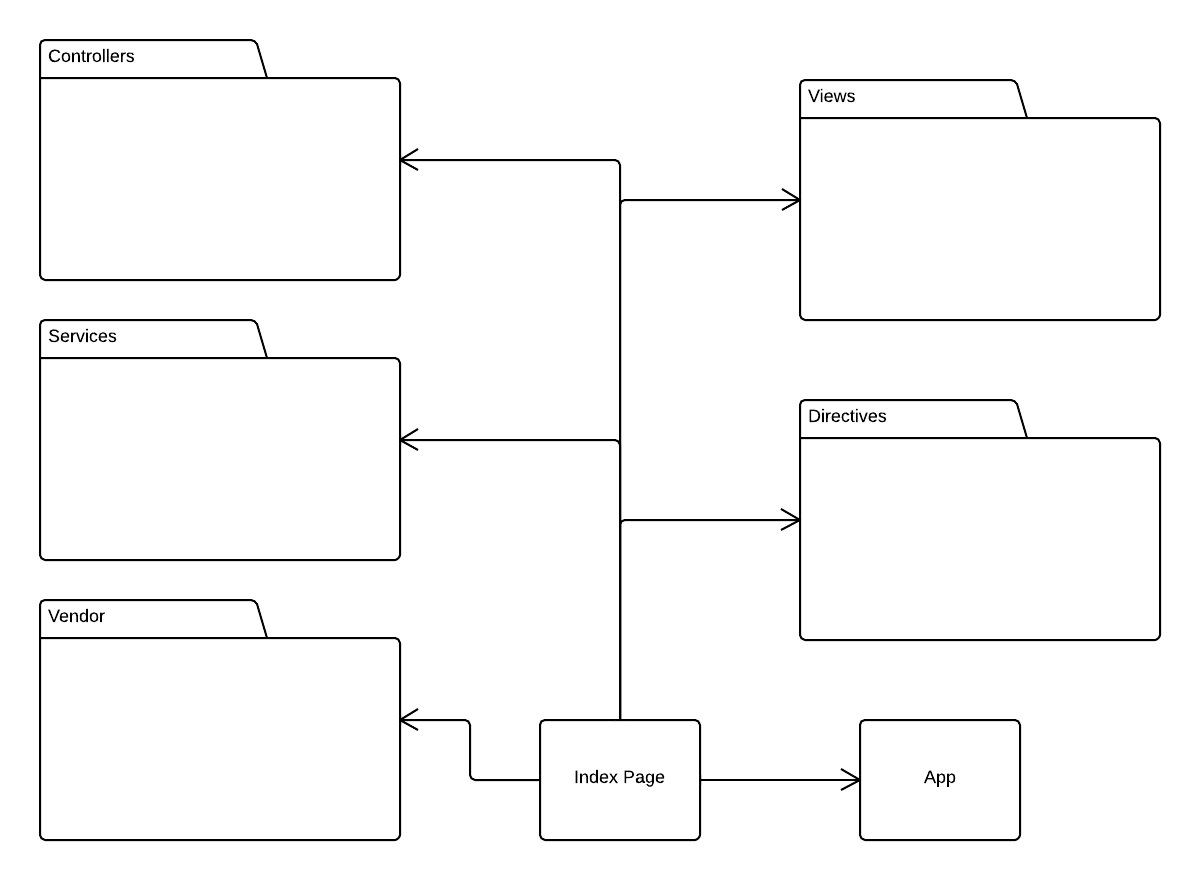
\includegraphics[width=0.8\linewidth]{./img/web-client-uml/subsystem-diagram}
\caption{Web client subsystem diagram.}
\label{fig:subsystem-diagram}
\end{figure}



\subsubsection{User Interfaces}
\label{sec:portal-user-interfaces}

This section presents and discusses the final user interfaces that were chosen for use in the web portal. These designs were the result of an iterative development process whereby the designs were shown to the client and revised according to suggested changes. They are also the result of interface enhancements designed to make the views more intuitive to users. The following sections will present a screen capture of each web portal view and discuss their functionality. The discussion for many of the interfaces remain the same as defined in the interim document and are cited as such.

\paragraph{Welcome View}\mbox{}\\
The welcome view shown in Figure \ref{fig:home} provides visitors with a link to download the Android application and instructs them to login or register account in order to use the portal. A footer has also been added to provide users with navigation links to important resources such as the Android application and \emph{About} page\cite{milestone2}.

\begin{figure}[H]

\centering

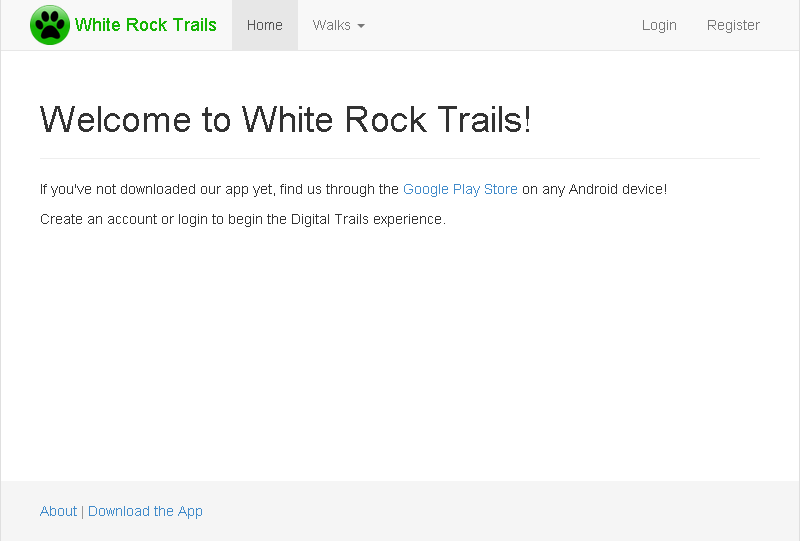
\includegraphics[width=1\linewidth]{./img/webportal/home}

\caption{Home view of the web portal.}

\label{fig:home}

\end{figure}



\paragraph{Responsive View}\mbox{}\\
Figure \ref{fig:home-responsive} demonstrates a responsive view of the web portal. This is the view that users will see when visiting the web portal on mobile devices such as smart phones and tablets. The responsive design minimizes the menu bar which can be expanded by clicking the button shown in the top right of the figure. In addition, web page content reduces in width and elements become stacked allowing for easier scrolling on mobile devices. The responsive design of the web portal is facilitated by the Bootstrap CSS and JavaScript library\cite{milestone2}. The items shown in the list feature navigational links to the associated pages. The \emph{Walks} item expands further child links which navigate to views that are associated with walks.



\begin{figure}[H]

\centering

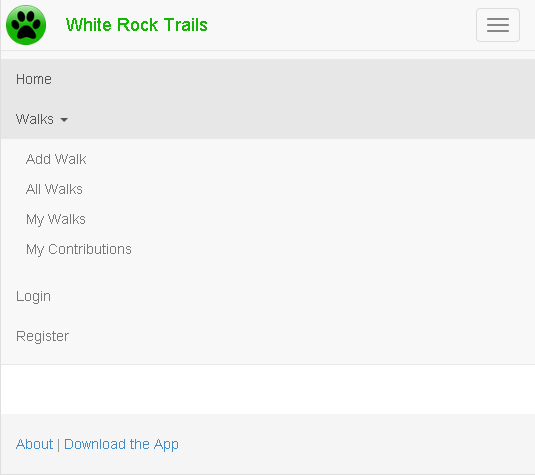
\includegraphics[width=1\linewidth]{./img/webportal/home-responsive}

\caption{Web portal responsive menu view.}

\label{fig:home-responsive}

\end{figure}



\paragraph{Login View}\mbox{}\\
Figure \ref{fig:login} shows the login view that users will see when they click on the \emph{Login} button in the top navigation bar. The login view displays as a modal in front of the web page. This will ensure that users do not have to navigate between pages in order to log in, thus enhancing usability. The login view requires users to input their email address and password followed by clicking the \emph{Login} button. The \emph{Login} button will display a spinner icon whilst the fields are validated to ensure the user is aware that the page is loading. An external validation library is used to validate the fields and display an error or success status. The library uses pre-defined validators to validate the structure of the email address and that the email and password pair is valid when checked against the White Rock Trails API. The validator changes the display of erroneous fields to feature red or green borders and tick or cross icons for invalid and valid fields respectively. A specific error message will also be displayed underneath erroneous fields to inform the reason for the error and allow users to amend it. When users successfully log in, the modal will close and the \emph{Login} and \emph{Registration} buttons shown in the top navigation bar are replaced with the user's full name\cite{milestone2}.



\begin{figure}[H]

\centering

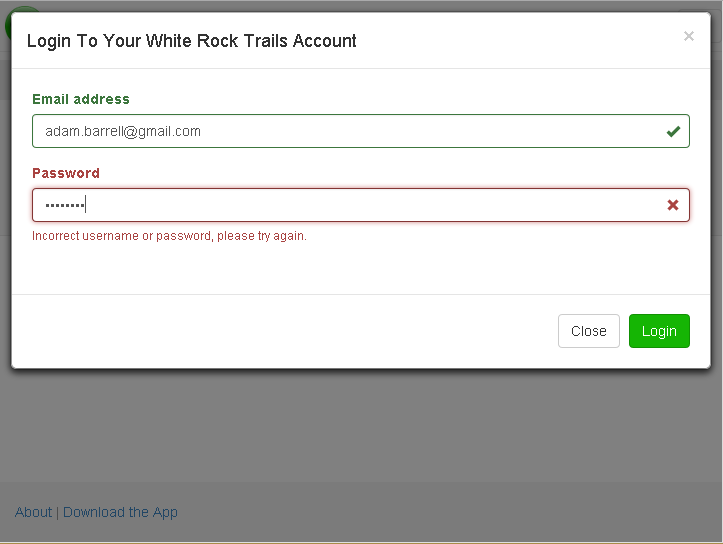
\includegraphics[width=0.7\linewidth]{./img/webportal/login}

\caption{Web portal login modal demonstrating validation.}

\label{fig:login}

\end{figure}



\paragraph{Registration View}\mbox{}
Figure \ref{fig:registration} shows the registration view that users will see when the \emph{Register} button is clicked in the top navigation bar. This view is also implemented as a modal for the same reasons as the login view and to maintain consistency throughout the application. The same validator is also used to validate the registration fields. However, inputs such as \emph{Email Address} and the two password fields require different validators. The former uses a validator that checks whether the provided email address has already been registered by another user. The latter checks whether the two passwords are identical. This will prevent users from registering using a mistyped password and subsequently not being able to log in. Clicking the \emph{Register} button will display a loading spinner inside as described for the login view. When users successfully register, they will be presented with a new confirmation modal instructing them to log in with their new account\cite{milestone2}.



\begin{figure}[H]

\centering

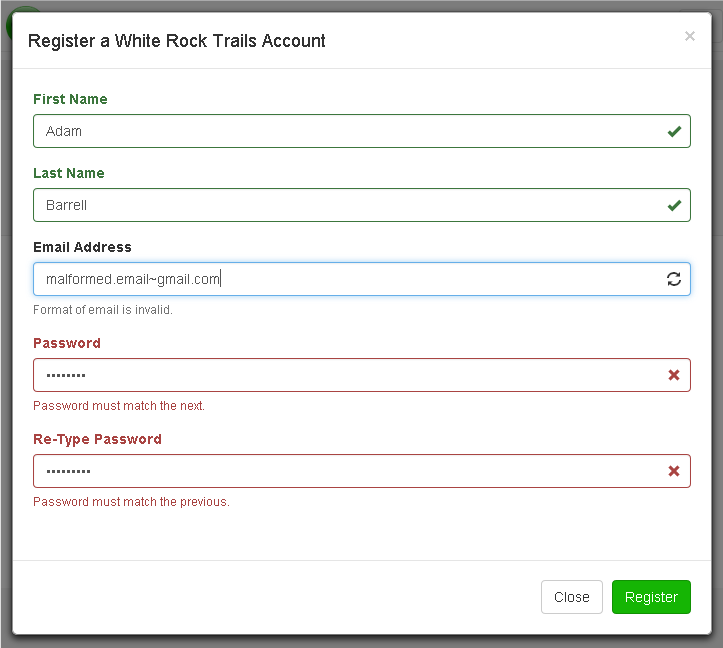
\includegraphics[width=0.7\linewidth]{./img/webportal/registration}

\caption{Web portal registration modal demonstrating validation.}

\label{fig:registration}

\end{figure}



\paragraph{All Walks View}\mbox{}\\
Figure \ref{fig:all-walks} shows the view users will see when they click on the \emph{Walks} button in the top menu bar and select the \emph{All Walks} option. This view displays a list of tiles, each representing a walk in the database. The background of each tile is an image selected from the collection of each walks way point images. Clicking a tile will navigate the user to a walk information view as presented in Figure \ref{fig:walk-info}\cite{milestone2}. 

Functionality for the \emph{Add Walk} button and search bar have been fully implemented since they were discussed in Milestone 2. Clicking the \emph{Add Walk} button navigates the user to a view where a new walk can be created. Entering text into the search box will perform a full text search of all walks held in the database. The search box also provides instantaneous results such that a request is sent to the server after a set time has expired after a user finishes typing. This allows for much faster and intuitive searching since the user is not required to press a button to execute the search. Finally, pagination has been implemented which allows users to view specific pages of search results that have overflowed the current view. A pagination control is present at the top and bottom of the \emph{All Walks} view for convenience to the user. Users can access specific results pages by clicking the relevant button index. 

\begin{figure}[H]

\centering

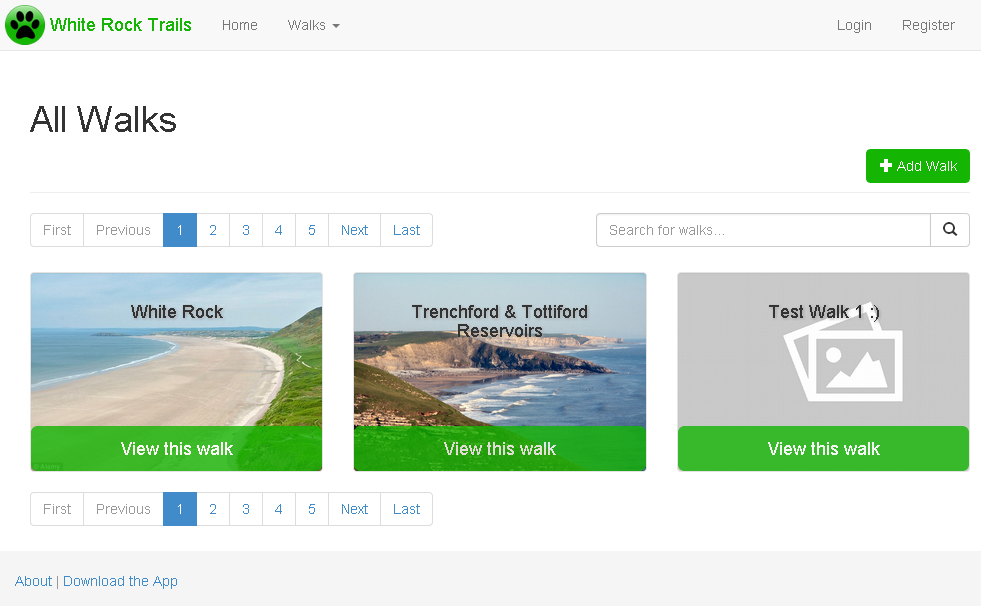
\includegraphics[width=1\linewidth]{./img/webportal/all-walks}

\caption{All walks view of the web portal.}

\label{fig:all-walks}

\end{figure}

\paragraph{Walk Information View}\mbox{}\\
Figure \ref{fig:walk-info} shows the view that a walk owner will see when they click on a walk owned by them from the \emph{All Walks} view. As shown in the figure, walk information will be displayed in this view such a title, description, duration, distance, difficulty rating and author. Navigation tabs above this information allow users to navigate between the \emph{Waypoints}, \emph{Reviews} and \emph{Walk} views. If any waypoint contributions have been submitted to the walk by other users, a \emph{Contributions} tab will appear. The number of pending contributions is also shown adjacent to the tab name. 

The interface also features \emph{Edit} and \emph{Delete} walk buttons which are only visible to the owner of the walk. Clicking the \emph{Edit} button will navigate the user to a view where the walk can be edited, whilst the \emph{delete} will prompt the user to confirm walk deletion. Walk data is asynchronously loaded from the database through the API. The Google Maps API is used to display the map shown in the right of the figure. The Google Maps API allows markers to be placed at specific GPS locations contained within the walk data. The map allows users to scroll and zoom around the walk area to gain an understanding of its location.

\begin{figure}[H]

\centering

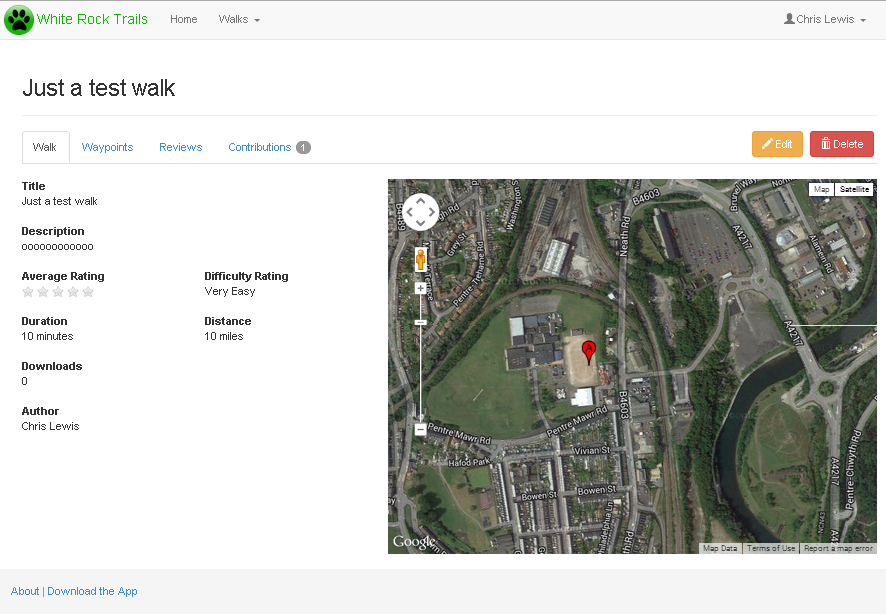
\includegraphics[width=1\linewidth]{./img/webportal/walk-info}

\caption{Walk information view of the web portal.}

\label{fig:walk-info}

\end{figure}

\paragraph{Walk Waypoints View}\mbox{}\\
Figure \ref{fig:walk-waypoints} shows the view that users will see when they click on the \emph{Waypoints} tab of the walk information view. The view shows the list of waypoints that are represented by markers on the map. Markers on the map can be identified by their letter index which references a waypoint shown in the leftmost list list. Clicking a list item or its corresponding map marker will display a modal containing media uploaded to the way point such as images, videos and audio. This feature has been fully implemented since Milestone 2. Finally, a visual fading effect has been applied to the waypoints list where an overflow is present. This indicates to the user that the list panel can be scrolled to display further waypoints.

\begin{figure}[H]

\centering

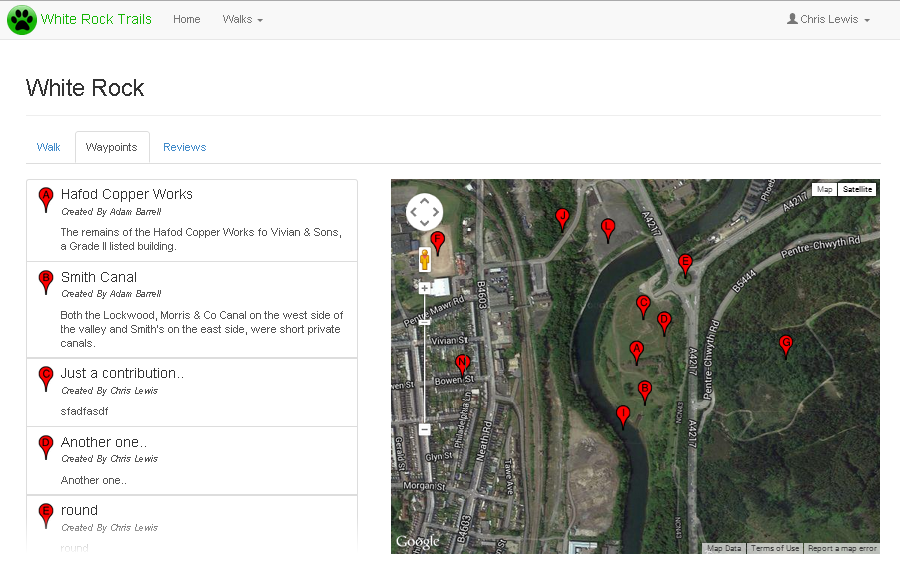
\includegraphics[width=1\linewidth]{./img/webportal/walk-waypoints}

\caption{Walk way points view of the web portal.}

\label{fig:walk-waypoints}

\end{figure}

\paragraph{Waypoint View}\mbox{}\\
The waypoint view shown in Figure \ref{fig:waypoint} is displayed when a list item or map marker is clicked from the walk waypoints view discussed in the previous paragraph. This view shows a read only representation of waypoint information such as its title, description and uploaded media. If the walk author is viewing this modal, an \emph{edit} and \emph{delete} button will be shown at the bottom which allows them to modify the waypoint. 

Clicking the \emph{edit} button will hide the current modal and display the waypoint in edit mode. Clicking the \emph{delete} button will prompt the user before permanently removing the waypoint from the walk. Clicking the final \emph{add image, audio or video} square in the gallery will allow the user to choose a file from their computer to be uploaded. Once chosen, the user will be required to enter a caption for the media. Upon specifying a caption, the media will be uploaded and added to the waypoint. 

Image and video media items are represented by a thumbnail image of their content. Since audio files do not have any visual representation, they have been given a gradient background featuring the caption above. The types of media displayed can be easily identified by an icon in the top left of each square. Clicking any media item will display a larger view the content and allow users to navigate backwards and forwards to previous and next media items respectively. This media viewer is presented in Figure \ref{fig:media-viewer}.

\begin{figure}[H]
\centering
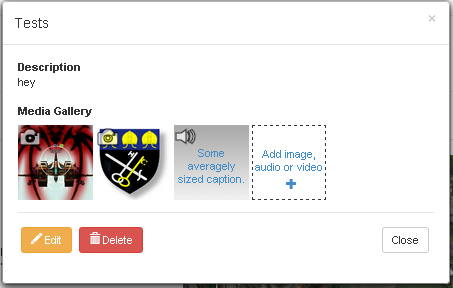
\includegraphics[width=0.7\linewidth]{./img/webportal/waypoint}
\caption{Walk waypoint view.}
\label{fig:waypoint}
\end{figure}

\begin{figure}[H]
\centering
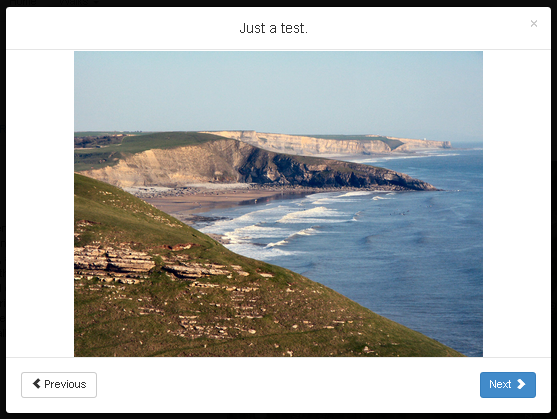
\includegraphics[width=0.7\linewidth]{./img/webportal/media-viewer}
\caption{Waypoint media viewer.}
\label{fig:media-viewer}
\end{figure}


\paragraph{Walk Reviews View}\mbox{}\\
Figure \ref{fig:walk-reviews} shows the view that users will see when they click the \emph{Reviews} tab from the navigation tabs bar. This view loads user reviews from the walk data and displays them in a list view as shown in the figure. A library called \emph{Raty} was used to generate the star rating system seen below the title of the review. It takes a review rating integer between 1-5 and generates a star representation\cite{milestone2}. Since Milestone 2, the review authors name now appears below the title so other users know who has created the review. In addition, authors of reviews will see a \emph{delete} button which can be clicked to remove their review. Walk owners will see the delete button on all reviews so to allow moderation.

Clicking the \emph{Add Review} button will hide the walk reviews and display a form which can be used to add a new one. When the user has submitted the new review, the list will re-appear and the form hidden.

\begin{figure}[H]
\centering
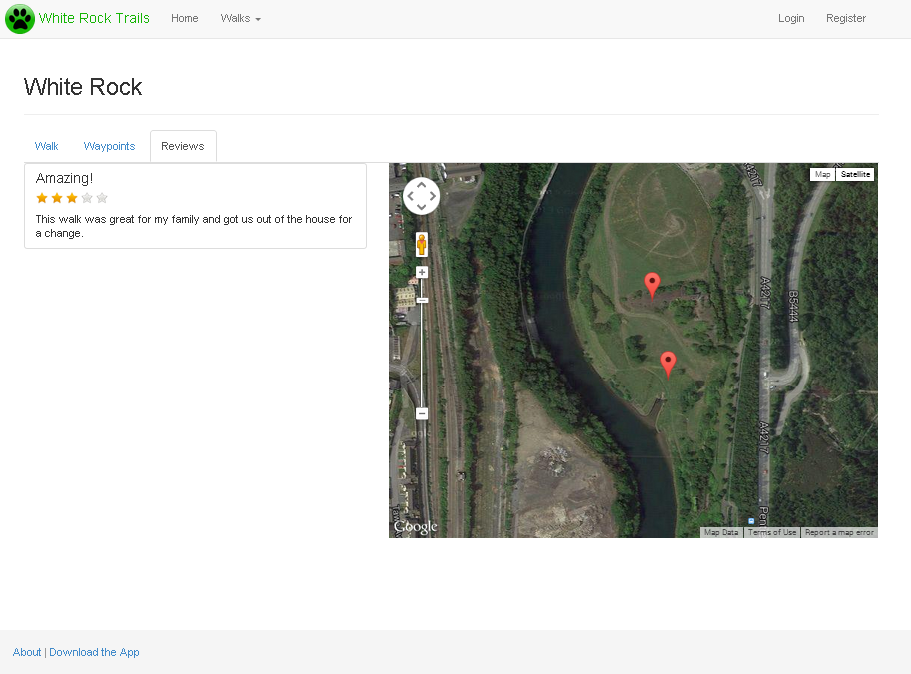
\includegraphics[width=1\linewidth]{./img/webportal/walk-reviews}
\caption{Walk reviews view of the web portal.}
\label{fig:walk-reviews}
\end{figure}

\paragraph{Waypoint Contributions View}\mbox{}\\
Since Milestone 2, an additional view has been added to allow walk authors to moderate waypoint contributions from other users. These will be displayed in a list as shown in Figure \ref{fig:waypoint-contributions}. Clicking a list item will present a modal displaying information about the waypoint that has been contributed. Each item has an \emph{accept} and \emph{reject} button to add the waypoint to the walk, or discard it respectively. Clicking either of these buttons will remove the contribution from the list and add a marker to the map representing its location.

\begin{figure}[H]
\centering
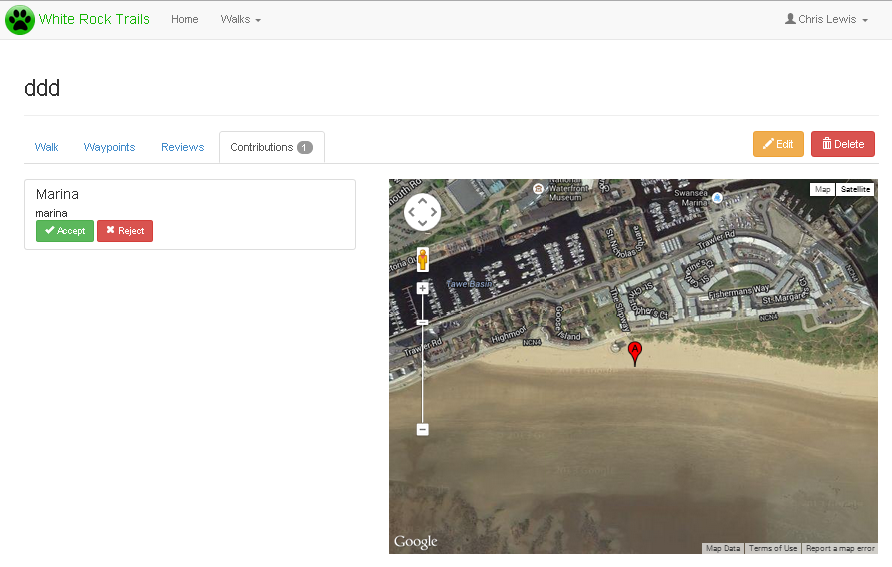
\includegraphics[width=1\linewidth]{./img/webportal/waypoint-contributions}
\caption{Waypoint contributions view.}
\label{fig:waypoint-contributions}
\end{figure}

\paragraph{Add Walk View}\mbox{}\\
The add walk view presented in Figure \ref{fig:add-walk} allows any user to create a new walk with associated waypoints. This view can be accessed from a link in the top navigation bar. Walk attributes can be entered and saved in the leftmost panel by clicking the \emph{save} button. The form can also be reset by clicking the \emph{undo} button. The \emph{cancel} button will discard the new walk and navigate back to the all walks view. The form also features client side error checking on saving, whereby erroneous fields are highlighted with a red border before the walk can be created. Waypoints can be added to the new walk by clicking on a map location. This will display the \emph{Add Waypoint} view discussed in the next paragraph.

\begin{figure}[H]
\centering
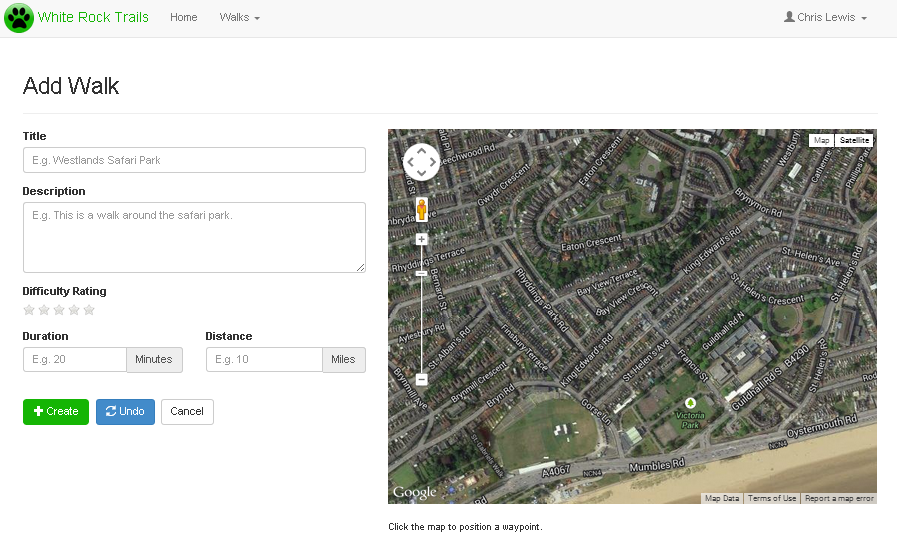
\includegraphics[width=1\linewidth]{./img/webportal/add-walk}
\caption{Add walk view.}
\label{fig:add-walk}
\end{figure}

\paragraph{Add Waypoint View}\mbox{}\\
The add waypoint view is presented in Figure \ref{fig:add-waypoint} and allows users to specify attributes of the waypoint to be created, including its \emph{title}, \emph{description}, \emph{latitude}, \emph{longitude}, \emph{visit order} and media. Clicking the \emph{Create} button will validate all fields and close the modal if successful. The waypoint will then be added to the new walk and a marker will appear on the map featured in the add walk view. Clicking the \emph{Manage} button will display an additional modal where media such as images, audio and videos can be added to the waypoint.

\begin{figure}[H]
\centering
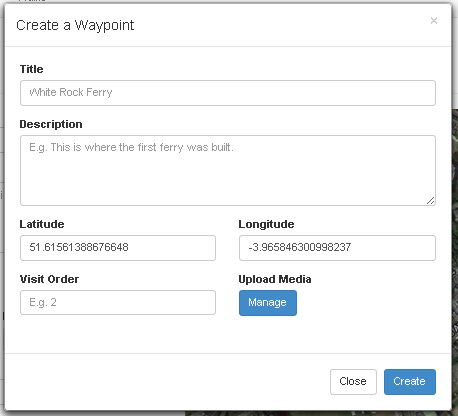
\includegraphics[width=0.7\linewidth]{./img/webportal/add-waypoint}
\caption{Add waypoint view.}
\label{fig:add-waypoint}
\end{figure}


\paragraph{Waypoint Media Gallery}\mbox{}\\
The waypoint media gallery shown in Figure \ref{fig:media-gallery} allows walk authors to manage the media which has been added to waypoints along their walks. Walk authors can select individual media items and click the \emph{delete selected} button to remove them in batch. Items selected for deletion are highlighted by a red border. The \emph{delete selected} button is only enabled when one or more media items are selected. On deleting media, they will be removed from the list and the \emph{delete selected} button disabled.

\begin{figure}[H]
\centering
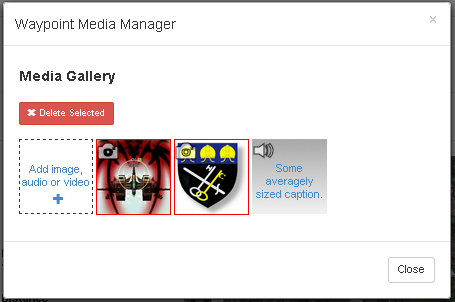
\includegraphics[width=0.7\linewidth]{./img/webportal/media-gallery}
\caption{Waypoint media gallery.}
\label{fig:media-gallery}
\end{figure}

\paragraph{Account Settings View}\mbox{}\\
The account settings view presented in Figure \ref{fig:user-account} allows registered users to modify their account details such as their \emph{first name}, \emph{last name}, \emph{email} and \emph{password}. All inputs are validated when the \emph{save} button is clicked. If any fields are invalid, they are given a red border to indicate this. Otherwise, a confirmation message is displayed above the account details to show the save has been successful.

\begin{figure}[H]
\centering
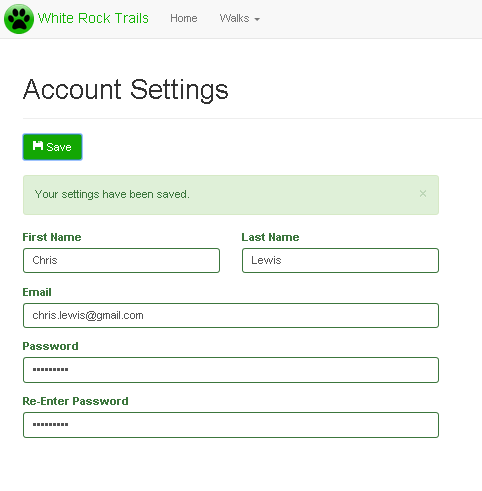
\includegraphics[width=0.7\linewidth]{./img/webportal/user-account}
\caption{User account settings view.}
\label{fig:user-account}
\end{figure}


\section{Android Application}
\label{sec:android-design}

\subsection{Technology Choices}
This section will discuss the choices of technology that were used to implement the application. These technologies were chosen for this project because both proved to be beneficial or essential to the development of the application. The following list will give the names of each technology and describe their purpose within the project.

\begin{itemize}

\item \textbf{Evolus Pencil} - Evolus Pencil is an open-source GUI prototyping tool that allows for mockups to be easily created. Pencil was used to create the initial prototype interface designs.

\item \textbf{Eclipse} - Eclipse is an integrated development environment that allows for the creation and development of applications. Eclipse was used to create the prototype designs for numerous interface iterations and the development of application functionality.

\end{itemize}

\subsection{User Interfaces}

\subsubsection{Rejected Designs}
\label{sec:rejected-designs}

Through-out the course of the project, many design iterations were carried out. As a result, numerous interface designs were modified, while several designs were made redundant for a variety of reasons. This section of the document will analyse rejected designs, highlighting the issues that led to their redundancy. Below is an example of how the interface designs have progressed through several stages of iteration.\\

\textbf{Choose a walk interface} - This example is the walk selection interface ``Saved Walks''. The first iteration took the form of a simple interface design (Figure \ref{fig:view_walk}). Created using Evolus Pencil, the interface included the majority of features set out by Milestone 1 requirements. Here, the user may select from a list of available walks. The main interface window presents the selected walk's name, geological location, description, length (miles) and number of walk waypoints. The interface also included a start button, allowing users to begin the walk in current view.

\begin{figure}[H]
    \centering
    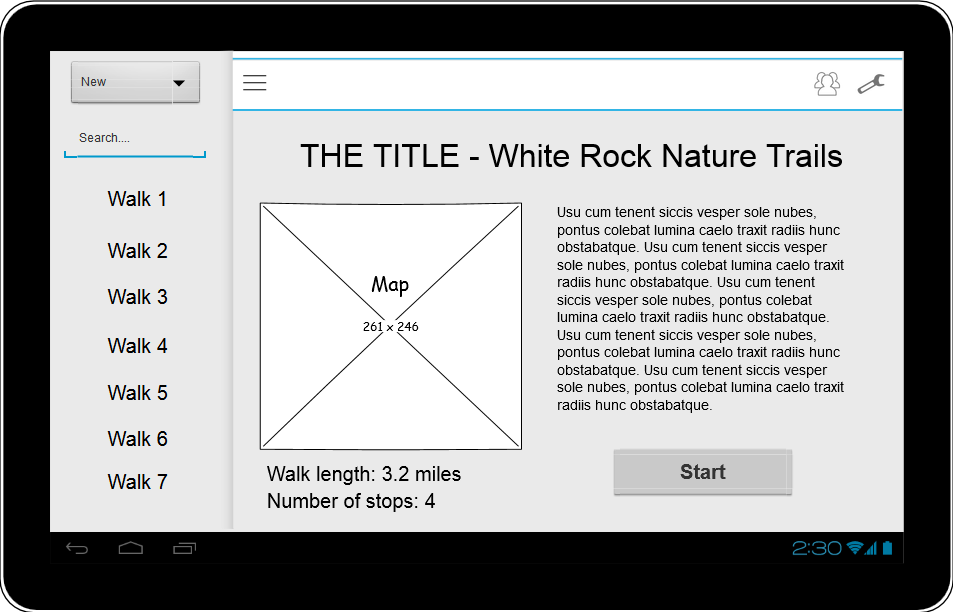
\includegraphics[width=0.8\textwidth]{chris/pencil_choose_walk}
    \caption{Walk selection interface - 1st iteration}
    \label{fig:choose_walk1}
\end{figure}

Based on the initial design, the interface was then created using Eclipse IDE [Cite]. This allowed for a more professional prototype design to be produced, illustrating how the final product may look. It was then possible to carry out improvements on the initial design. The \emph{combo-box} and \emph{search} features situated above the list of walks were removed. This was due to the fact they were better suited else where in the application, in a separate search interface. The removal of these two features now allowed for the list of walks to fill the entire side bar fragment. The final stage of this iteration was to add colour to the design. The chosen colour scheme for this iteration was a light shade of green to compliment the application logo. A small amount of shading was applied to the background colour of buttons and other features. 

\begin{figure}[H]
    \centering
    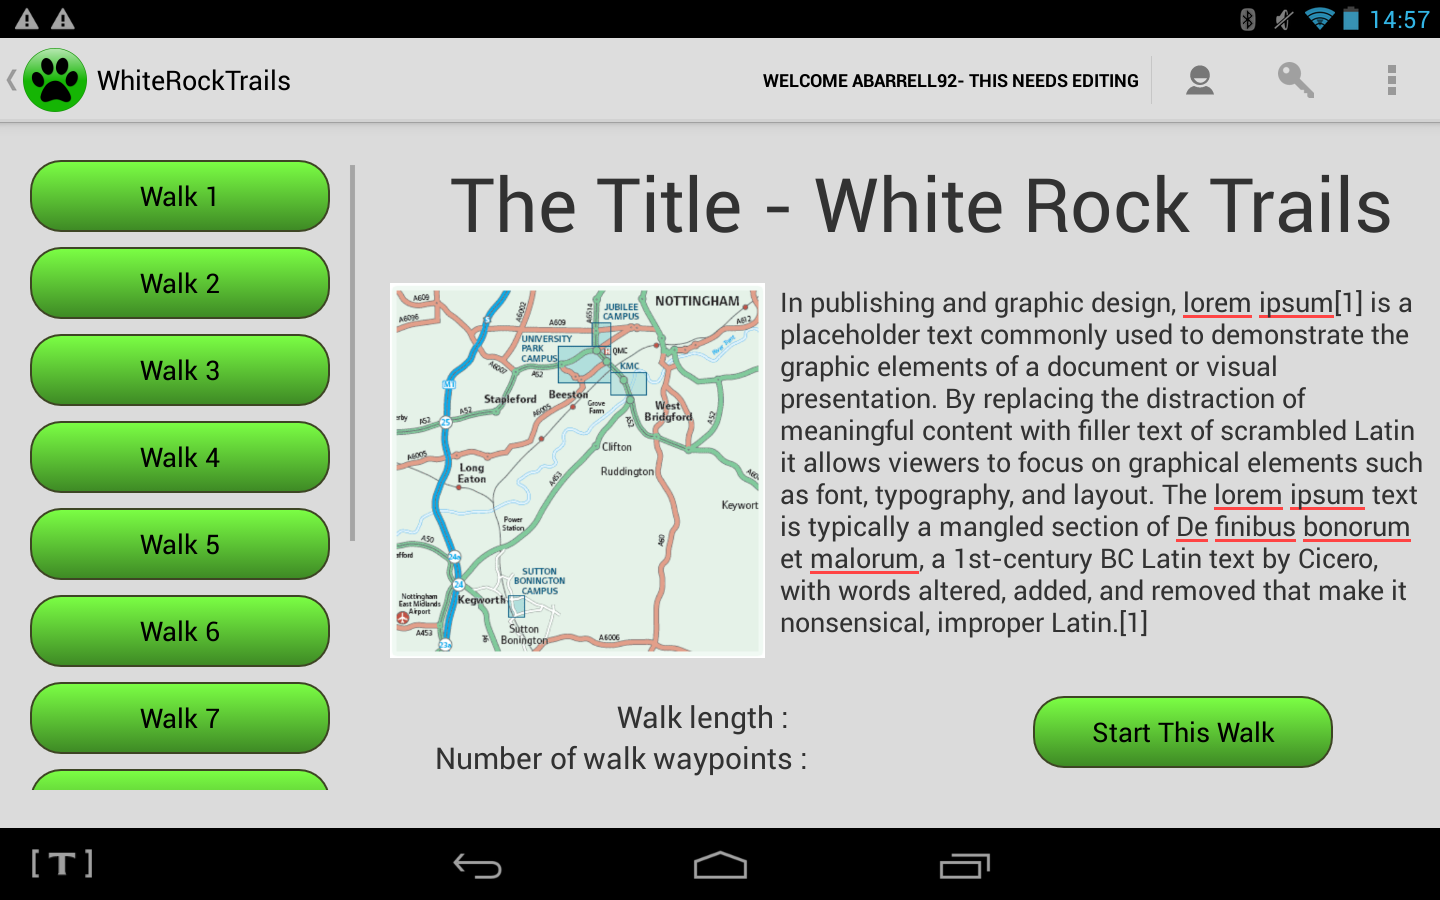
\includegraphics[width=0.8\textwidth]{chris/app_choose_walk}
    \caption{Walk selection interface - 2nd iteration}
    \label{fig:choose_walk2}
\end{figure}

The final iteration involved several layout alterations (Figure \ref*{fig:choose_walk3}). First, the list of walks fragment button style was removed. This was replaced by a walk list that was read from a database. The \emph{walk title} and \emph{description} are also now read from the database, and provide prompt text when the interface is first inflated. The \emph{start walk} button was raised to be aligned with the bottom of the walk map. Two additional features were also implemented. An \emph{average rating} star system was introduced along with a \emph{difficulty rating}. Both rating features are based on user feedback.

\begin{figure}[H]
    \centering
    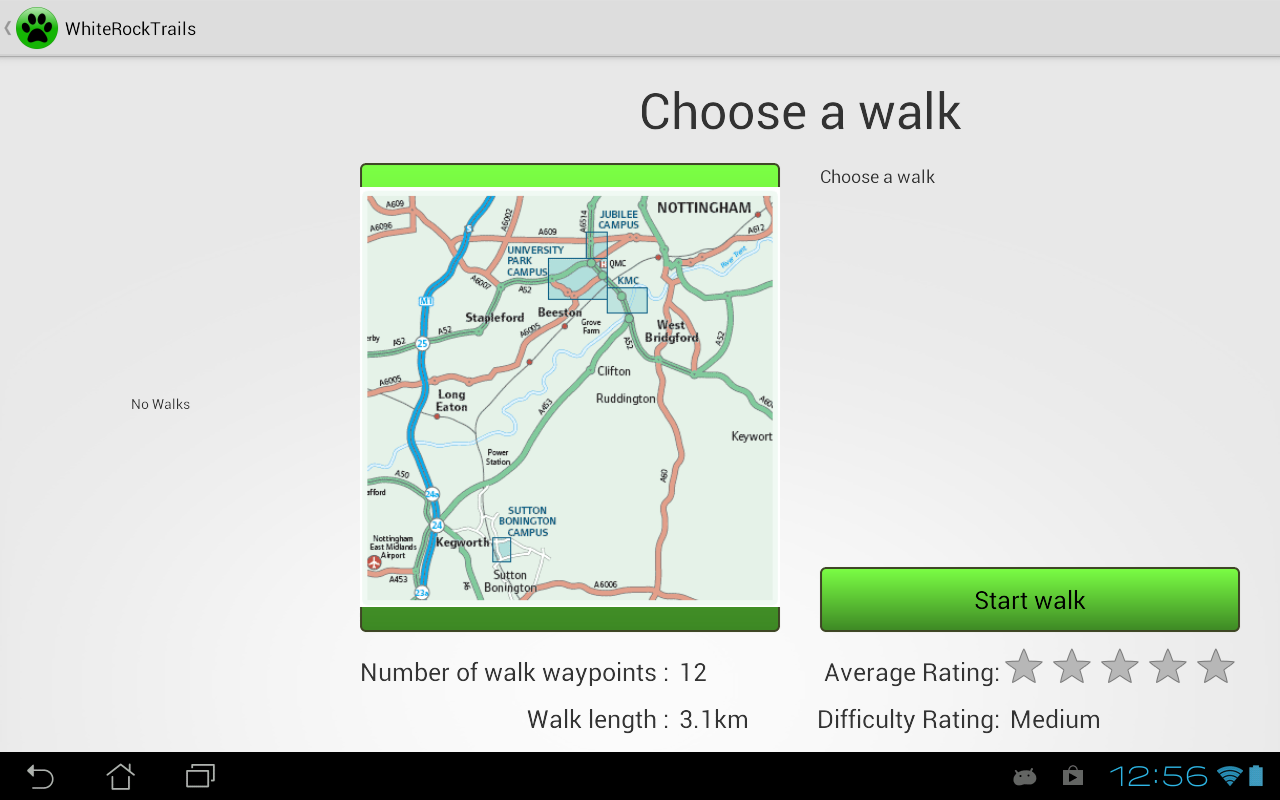
\includegraphics[width=0.8\textwidth]{chris/final_choose_walk}
    \caption{Walk selection interface - 3rd iteration EDIT THIS FOR WORKING MAP}
    \label{fig:choose_walk3}
\end{figure}


As previously documented, many interface designs were altered during the iteration stages of development. However, a small number of interface designs were fully rejected and re-designed. Below is a similar example of complete interface re-designs.\\

\textbf{My Walks interface} - The second design iteration saw the ``My Walks'' interface (Figure~\ref{fig:app_my_walks_view1}) present each walk create by the user in list form. Each walk included an \emph{ID}, \emph{title}, \emph{edit} and \emph{delete} button. The user also had the ability to create a new walk from this interface. During evaluation, it was decided that the proposed interface was not suitably designed. It's inappropriate layout meant that the only information available about each walk was in fact its ID and title. Before selecting the edit or delete button, the user may have to view a walk if they were unable to recall by name. The list format also led to a poor use of layout positioning. A vast amount of empty space was visible, especially when using the application on a large tablet.

\begin{figure}[H]
    \centering
    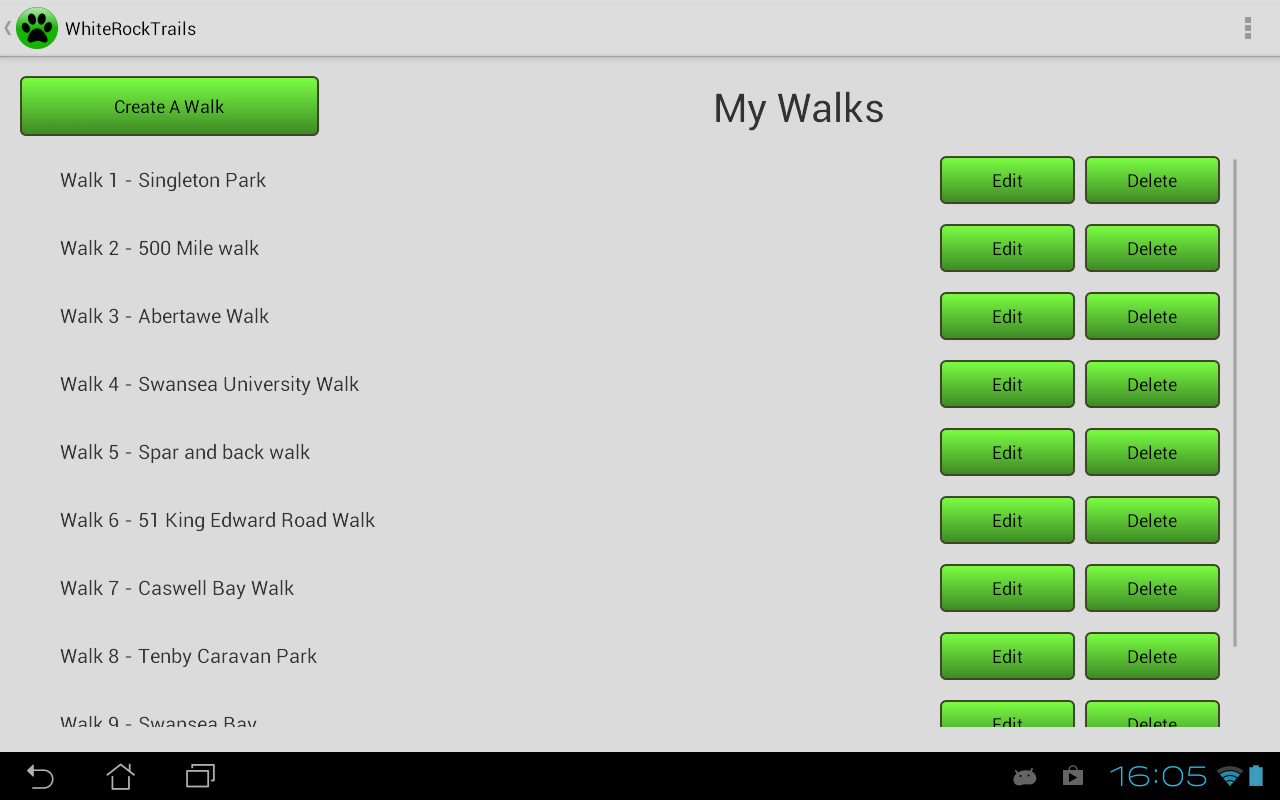
\includegraphics[width=0.8\textwidth]{chris/app_my_walks_view}
    \caption{My Walks interface - 2nd iteration}
    \label{fig:app_my_walks_view1}
\end{figure}

With the above negative aspects of this design taken into consideration, a new interface design was produced (Figure \ref{fig:app_my walks_view2}). The interface now presents each walk in a side-bar style list fragment, reading each walk from a database. The \emph{edit} and \emph{delete} buttons are included in the main fragment. Additional features to the interface now include the walk's \emph{geological location}, \emph{description}, \emph{length(in miles)}, \emph{number of walk waypoints}, \emph{difficulty rating} and \emph{average user rating}. Providing this level of information allows users to view a basic summary of each walk created by the user.\\

\begin{figure}[H]
    \centering
    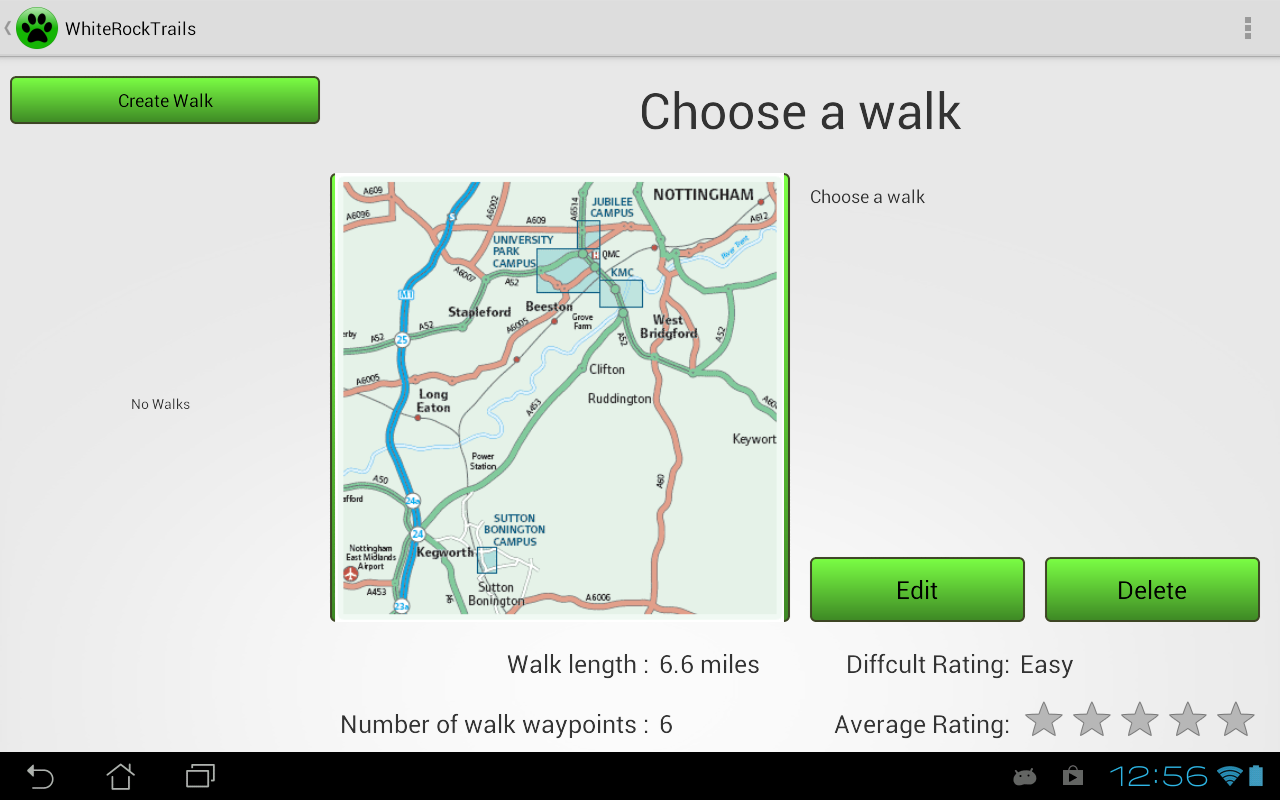
\includegraphics[width=0.8\textwidth]{chris/final_walk_view}
    \caption{My Walks interface - 3rd iteration}
    \label{fig:app_my walks_view2}
\end{figure}
% User Interface Design
% UML Diagrams
% Descriptions of each class
% Technology Choices

\subsubsection{Chosen Design}
\label{sec:chosen-designs}

This section presents and discusses the final user interfaces that were chosen for use in the application. These designs were the result of an iterative development process whereby the designs were shown to the client and revised according to suggested changes. They are also the result of interface enhancements, designed to make each interface more intuitive to users. The following sections will present a screen capture of each interface application and discuss their functionality.

\paragraph{Splash Screen interface}\mbox{}\\ 
INSERT IMAGE\\

The \emph{splash screen} is the first interface inflated when the application is opened. It includes the company logo, company name and a loading feature. After a short period of time, the \emph{launch} interface will inflate.

\paragraph{Launch interface}\mbox{}\\
INSERTT IMAGE\\

The \emph{launch} interface presents the user with an aesthetically pleasing layout. An edited image of the local beach is used as the background. At the top of the interface is a \emph{Text View} welcoming the user to the application. At the centre of the interface is a \emph{Log In}. Pressing the \emph{Log in} button will navigate to the \emph{Log In} interface. A \emph{Continue as guest} button is also situated at the bottom right corner. Pressing this button will by-pass the log in feature and take the user directly to the \emph{Home} interface but with limited privileges.

\paragraph{Log In interface}\mbox{}\\
INSERTT IMAGE\\

The \emph{Log In} interface presents the user with a welcome message fixed to the top, along with prompt text directly below. The focus of this interface is the \emph{email} and \emph{password} text boxes. Selecting either text box will inflate a keypad, where the user may enter log in details. Below is a \emph{Sign In} button and a \emph{New user?} text view. If valid details are entered, pressing the \emph{Sign In} button will navigate to the \emph{Home} interface. If invalid details are entered, a pop-up dialogue will notify users that the log in attempt has failed. Pressing the \emph{New user?} text view will navigate to the \emph{Register} interface, where the user may register a new account.

\paragraph{Register interface}\mbox{}\\
INSERTT IMAGE\\

The \emph{Register} interface presents the user with a series of edit text boxes, where details such as \emph{first name, last name, email address} and \emph{password} can be entered in order to create a new account. Below this is a \emph{Create Account} button and an \emph{Already a member?} text view. If suitable details are entered, pressing the \emph{Create Account} button will create a user account and navigate to the \emph{Home} interface. If unsuitable, the account creation will be rejected.

\paragraph{Home interface}\mbox{}\\
INSERTT IMAGE\\

The \emph{Home} interface is the central focus point of the application. This interface includes a title and a grid of four navigation buttons; a \emph{Saved Walks}, a \emph{Download Walks}, a \emph{My Walks} and an \emph{Explore} button. Pressing on any button will navigate to the respective interface.

\paragraph{Saved Walks interface}\mbox{}\\
INSERTT IMAGE\\

The \emph{Saved Walks} interface presents a list of all saved walks on the left hand side. The main interface window displays the \emph{walk title, description, geological location} map and a \emph{start} button. Pressing the \emph{start} button will inflate a map interface and begin the walk trail.

\section{API} 
\label{sec:api-design}

The API is the crucial link between the Website, Application and Database. It was important that the correct design and technology was selected to make that link as seamless as possible. 

\subsection{Technology Choices}
\label{sec:api:techChoices}

\begin{description}
\item[Paris] - Paris is an ORM (Object Relation Mapper) which provided a layer of abstraction between the database and the API. Rather than writing SQL queries to retrieve an object it makes it possible to use model objects to and methods to retrieve the objects.  
\item[Slim Framework] - The slim framework was chosen as the underlying framework of the API. Slim provides many low-level function which are critical to the production of a reliable API in a small and efficient package. Before it was settled on an alternative framework called Phalcon was trialed, but it proved to be overly complex and overwhelming compared to the relative simplicity of Slim. 
\item[PHP] - This is the language on which Slim runs. It is a popular free and open source web programming langauage. It has great support and is widly used through the world. Alternatives included C\#.NET which is a closed source and closed platform product from Microsoft. Due to the licensing fees and extra costs involved PHP quickly came to light as the best choice. 
\item[Apache] - This is the web server which handles request and responses for the API. It recieves requests and passes them on to the PHP runtime for the API. Apache is the best known and most widely used web server in the world. The alternatives were Nginx and IIS. IIS is limited to Microsfts platforms and Nginx, while well respected, is still an emerging presence in the market. 
\item[Linux] - Linux is the operating system which powers the API server. Linux is free and open source and is the most popular platfrom for operating a server.
\item[JSON] - JavaScript Object Notation (JSON) is a media format which is used to represent JavaScript objects as plain text. It can be used to represent far more than just JavaScript objects however. 
\end{description}

\subsection{Possible Designs}
\label{sec:api:rejected-designs} %Phalcon Framework. SOAP API's.
When work started on the API the first descision that needed to be made was on the protocal for the API. There are several popular API protocals including;

\begin{itemize}
\item SOAP
\item REST
\item JSON-RPC 
\item XML-RPC \ldots
\end{itemize}

The most popular two are SOAP and REST. SOAP was originally defined as `Simple Object Access Protocol' and is the sucssesor to XML-RPC (XML Remote Procedure Call). It uses a XML document for its message which is sent over either the HTTP or SMTP application protocals. The XML document which is transmitted with a SOAP request has several parts. The document will start with an `Envelope' which contains all of the data. Inside the `Envelope' there is an optional `Header', a compolsary `Body' which contains request data, and an optional `Fault' which contains any errors which have occured. Listing \ref{lst:soap} shows an example of a SOAP request.

\lstset{language=xml,
keywordstyle=\color{Maroon},
commentstyle=\color{OliveGreen},
showstringspaces=false, tabsize=4, breaklines=true, showspaces=false, stringstyle=\color{Blue}}

\begin{lstlisting}[captionpos=b, caption=An example SOAP request., label=lst:soap, frame=single]
POST /InStock HTTP/1.1
Host: www.example.org
Content-Type: application/soap+xml; charset=utf-8
Content-Length: 299
SOAPAction: "http://www.w3.org/203/05/soap-envelope"
 
<?xml version="1.0"?>
<soap:Envelope xmlns:soap="http://www.w3.org/203/05/soap-envelope">
  <soap:Header>
  </soap:Header>
  <soap:Body>
    <m:GetStockPrice xmlns:m="http://www.example.org/stock">
      <m:StockName>IBM</m:StockName>
    </m:GetStockPrice>
  </soap:Body>
</soap:Envelope>
\end{lstlisting}

REST, on the other hand, is a stateless system which comunicates via URI's, any media (such as JSON or XML) and HTTP Methods. REST stands for Representational State Transfer, which implys a representation of the current state must be transfered to the API with reach request. A REST request to retrive an object can be as simple as \lstinline$GET http:\\example.com\api\users$. The simplicity of REST lends its self to many situations and makes it easy to adapt to specific cases. 

\subsection{Chosen Desgin}
For the API it was decided to harness the REST protocal. The decision was made after analysing both SOAP and REST and the advantages and disadvantages of both. In the end the overly veribose nature of SOAP led to the decision of a REST api.  The ability to use JSON with REST requests was also a deciding factor as this gretly reduced the workload when comunicating with the API from JavaScript. 

\subsection{Classes}
\label{sec:api:class}
The API has several `Model' classes to represent the Database tables and the objects that are stored within them. The objects are related through the database and can retrieve the related models through method calls. The relations between the models is shown in Figure \ref{fig:datamodels}, where every model is a possible entry point. Using these models it is possible to, for example, use an `English Walk Description' to return all related 'Waypoint Images'. 

\begin{figure}[H]
    \centering
    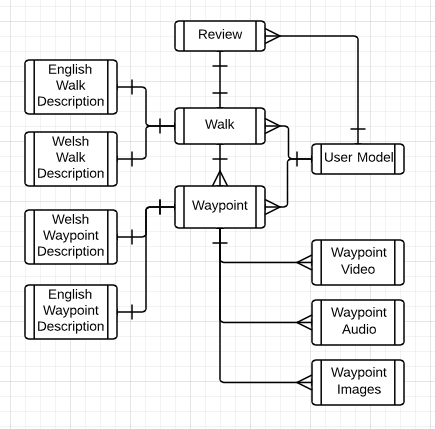
\includegraphics[width=0.5\textwidth]{DataModels}
    \caption{The Data Model and their relations.}
    \label{fig:datamodels}
\end{figure}

The API has several main object collections, which are `Walks', `Waypoints', `Users', `Waypoint Images', `Waypoint Audio', `Waypoint Video', `Walk Reviews' and `Sessions'. Each collection has a specific route in the API which maps to a collection controller. When a route is called a method in the revelvent controller is called. The method is passed a variable called \$app. This contains the requets and response objects. When the controller has completed its work it writes the response to the \$app object and returns to the index file which initally handled the request. If there is no more work to be done the \$app object sends the response. 

\begin{figure}[H]
    \centering
    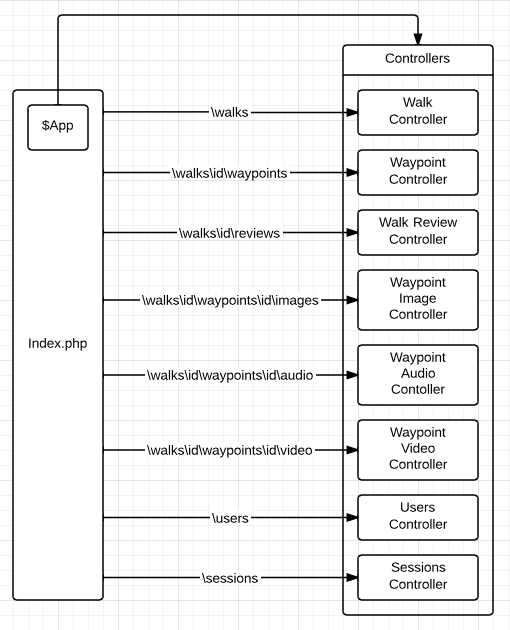
\includegraphics[width=0.5\textwidth]{ControllerRoutes}
    \caption{The connection between routes and controllers.}
    \label{fig:controllerroutes}
\end{figure}

Each controller has methods to respond to diffrent requests, a generic controller will have `getOne', `getAll', `add', `update', `remove' and `search'. The methods match up to specific routes. For example `getOne' normally matches to \textbf{GET} \url{/resources/id} and `add' matches \textbf{POST} \url{/resources}. 

\subsubsection{Walk Controller}

The walk controller process request for several diffrent functions. It provides the most functionality allowing not just for traditional CRUD operations but also for searching. 

\begin{table}[H]
\centering
\begin{tabular}{l | l | l}
HTTP Method & Route & Contorller Method\\ \hline
\textbf{\textcolor{Maroon}{GET}} & \url{/walks} & \lstinline$getAll()$ \\
\textbf{\textcolor{Maroon}{GET}} & \url{/walks/}\bfurl{id} & \lstinline$getOne(id)$\\
\textbf{\textcolor{Maroon}{POST}} & \url{/walks} & \lstinline$add()$\\
\textbf{\textcolor{Maroon}{PUT}} & \url{/walks/}\bfurl{id} & \lstinline$update(id)$\\
\textbf{\textcolor{Maroon}{DELETE}} & \url{/walks/}\bfurl{id} & \lstinline$delete(id)$\\
\textbf{\textcolor{Maroon}{GET}} & \url{/walks/search/}\bfurl{query} & \lstinline$search(query)$\\
\end{tabular}
\caption{Routes and Methods in the Walks Controller}
\label{tab:walksController}
\end{table}

\subsubsection{Waypoint Controller}

The waypoint contorller provides the basic CRUD operations. When adding or getting all waypoints it requires the id of the walk they should belong to. When acting upon an individual waypoint it needs the waypoints id, called \bfurl{wid} in the table. 

\begin{table}[H]
\centering
\begin{tabular}{l | l | l}
HTTP Method & Route & Contorller Method\\ \hline
\textbf{\textcolor{Maroon}{GET}} & \url{/walks/}\bfurl{id}\url{/waypoints} & \lstinline$getAll(id)$ \\
\textbf{\textcolor{Maroon}{GET}} & \url{/walks/}\bfurl{id}\url{/waypoints/}\bfurl{wid} & \lstinline$getOne(wid)$\\
\textbf{\textcolor{Maroon}{POST}} & \url{/walks/}\bfurl{id}\url{/waypoints} & \lstinline$add(id)$\\
\textbf{\textcolor{Maroon}{PUT}} & \url{/walks/}\bfurl{id}\url{/waypoints/}\bfurl{wid} & \lstinline$update(wid)$\\
\textbf{\textcolor{Maroon}{DELETE}} & \url{/walks/}\bfurl{id}\url{/waypoints/}\bfurl{wid} & \lstinline$delete(wid)$\\
\end{tabular}
\caption{Routes and Methods in the Waypoint Controller}
\label{tab:waypointController}
\end{table}

\subsubsection{Walk Review Controller}

The walk review controller allows the user to get all reivews for a walk, get an idividual review, add a review to a walk and delete a review. Users are prohibited from updating a review once it has been submitted. Users are expected to pass a valid walk object in JSON when they add and will recieve back valid objects with every request. 

\begin{table}[H]
\centering
\begin{tabular}{l | l | l}
HTTP Method & Route & Contorller Method\\ \hline
\textbf{\textcolor{Maroon}{GET}} & \url{/walks/}\bfurl{id}\url{/reviews} & \lstinline$getAll(id)$ \\
\textbf{\textcolor{Maroon}{GET}} & \url{/walks/}\bfurl{id}\url{/reviews/}\bfurl{rid} & \lstinline$getOne(rid)$\\
\textbf{\textcolor{Maroon}{POST}} & \url{/walks/}\bfurl{id}\url{/reviews} & \lstinline$add(id)$\\
\textbf{\textcolor{Maroon}{DELETE}} & \url{/walks/}\bfurl{id}\url{/reviews/}\bfurl{rid} & \lstinline$delete(rid)$\\
\end{tabular}
\caption{Routes and Methods in the Walk Revew Controller}
\label{tab:waypointController}
\end{table}

\subsubsection{Waypoint Image Controller}

Waypoint Image Controller allows users to upload images for waypoints. Users are able to add, remove and get images (Either all of them or jsut one). When uploading a file the request should contain the file, which is then moved within the server and stored and a thumbnail is generated. 

\begin{table}[H]
\centering
\begin{tabular}{l | l | l}
HTTP Method & Route & Contorller Method\\ \hline
\textbf{\textcolor{Maroon}{GET}} & \url{/walks/}\bfurl{id}\url{/waypoints/}\bfurl{wid}\url{/images} & \lstinline$getAll(wid)$ \\
\textbf{\textcolor{Maroon}{GET}} & \url{/walks/}\bfurl{id}\url{/waypoints/}\bfurl{wid}\url{/images/}\bfurl{img_id} & \lstinline$getOne(img_id)$\\
\textbf{\textcolor{Maroon}{POST}} & \url{/walks/}\bfurl{id}\url{/waypoints/}\bfurl{wid}\url{/images} & \lstinline$add(wid)$\\
\textbf{\textcolor{Maroon}{DELETE}} & \url{/walks/}\bfurl{id}\url{/waypoints/}\bfurl{wid}\url{/images/}\bfurl{img_id} & \lstinline$delete(wid)$\\
\end{tabular}
\caption{Routes and Methods in the Waypoint Image Controller}
\label{tab:waypointImageController}
\end{table}

\subsubsection{Waypoint Audio Controller}

Waypoint Audio Controller is similar to the image controller, it allows users to upload audio for waypoints. Users are able to add, remove and get audio samples (Either all of them or jsut one). When uploading a file the request should contain the file, which is then moved within the server and stored. 

\begin{table}[H]
\centering
\begin{tabular}{l | l | l}
HTTP Method & Route & Contorller Method\\ \hline
\textbf{\textcolor{Maroon}{GET}} & \url{/walks/}\bfurl{id}\url{/waypoints/}\bfurl{wid}\url{/images} & \lstinline$getAll(wid)$ \\
\textbf{\textcolor{Maroon}{GET}} & \url{/walks/}\bfurl{id}\url{/waypoints/}\bfurl{wid}\url{/images/}\bfurl{img_id} & \lstinline$getOne(img_id)$\\
\textbf{\textcolor{Maroon}{POST}} & \url{/walks/}\bfurl{id}\url{/waypoints/}\bfurl{wid}\url{/images} & \lstinline$add(wid)$\\
\textbf{\textcolor{Maroon}{DELETE}} & \url{/walks/}\bfurl{id}\url{/waypoints/}\bfurl{wid}\url{/images/}\bfurl{img_id} & \lstinline$delete(wid)$\\
\end{tabular}
\caption{Routes and Methods in the Waypoint Audio Controller}
\label{tab:waypointAudioController}
\end{table}

\subsubsection{Waypoint Video Controller}

Waypoint Video Controller is very similar to the image controller. Users are able to add, remove and get videos (Either all of them or jsut one). When uploading a file the request should contain the file, which is then moved within the server and stored and a thumbnail is generated. 

\begin{table}[H]
\centering
\begin{tabular}{l | l | l}
HTTP Method & Route & Contorller Method\\ \hline
\textbf{\textcolor{Maroon}{GET}} & \url{/walks/}\bfurl{id}\url{/waypoints/}\bfurl{wid}\url{/images} & \lstinline$getAll(wid)$ \\
\textbf{\textcolor{Maroon}{GET}} & \url{/walks/}\bfurl{id}\url{/waypoints/}\bfurl{wid}\url{/images/}\bfurl{img_id} & \lstinline$getOne(img_id)$\\
\textbf{\textcolor{Maroon}{POST}} & \url{/walks/}\bfurl{id}\url{/waypoints/}\bfurl{wid}\url{/images} & \lstinline$add(wid)$\\
\textbf{\textcolor{Maroon}{DELETE}} & \url{/walks/}\bfurl{id}\url{/waypoints/}\bfurl{wid}\url{/images/}\bfurl{img_id} & \lstinline$delete(wid)$\\
\end{tabular}
\caption{Routes and Methods in the Waypoint Video Controller}
\label{tab:waypointVideoController}
\end{table}

\subsubsection{User Controller}

The User Controller allows users to get users (Either all or just one), allows user to be added (Registration), allows users to be searched for and lets uses update or delete their own account. If a user trys to modify or delete an account that is no their own the controller will block the request and return a 403 Forbiden error. 

\begin{table}[H]
\centering
\begin{tabular}{l | l | l}
HTTP Method & Route & Contorller Method\\ \hline
\textbf{\textcolor{Maroon}{GET}} & \url{/users} & \lstinline$getAll()$ \\
\textbf{\textcolor{Maroon}{GET}} & \url{/users/}\bfurl{id} & \lstinline$getOne(id)$\\
\textbf{\textcolor{Maroon}{POST}} & \url{/users} & \lstinline$add()$\\
\textbf{\textcolor{Maroon}{PUT}} & \url{/users/}\bfurl{id} & \lstinline$update(id)$\\
\textbf{\textcolor{Maroon}{DELETE}} & \url{/users/}\bfurl{id} & \lstinline$delete(id)$\\
\textbf{\textcolor{Maroon}{GET}} & \url{/users/search/}\bfurl{query} & \lstinline$search(query)$\\
\end{tabular}
\caption{Routes and Methods in the User Controller}
\label{tab:usersController}
\end{table}

\subsubsection{Session Controller}

The session controller provides only two features, login and logout. Login will assign the user an authorisation token to authenticate their requests and logout will remove that auth token from the user. 

\begin{table}[H]
\centering
\begin{tabular}{l | l | l}
HTTP Method & Route & Contorller Method\\ \hline
\textbf{\textcolor{Maroon}{POST}} & \url{/sessions} & \lstinline$login()$\\
\textbf{\textcolor{Maroon}{DELETE}} & \url{/sessions} & \lstinline$logout()$\\
\end{tabular}
\caption{Routes and Methods in the Session}
\label{tab:SessionController}
\end{table}

\section{The Database}
\label{sec:database-design}

\begin{figure}[H]
    \centering
    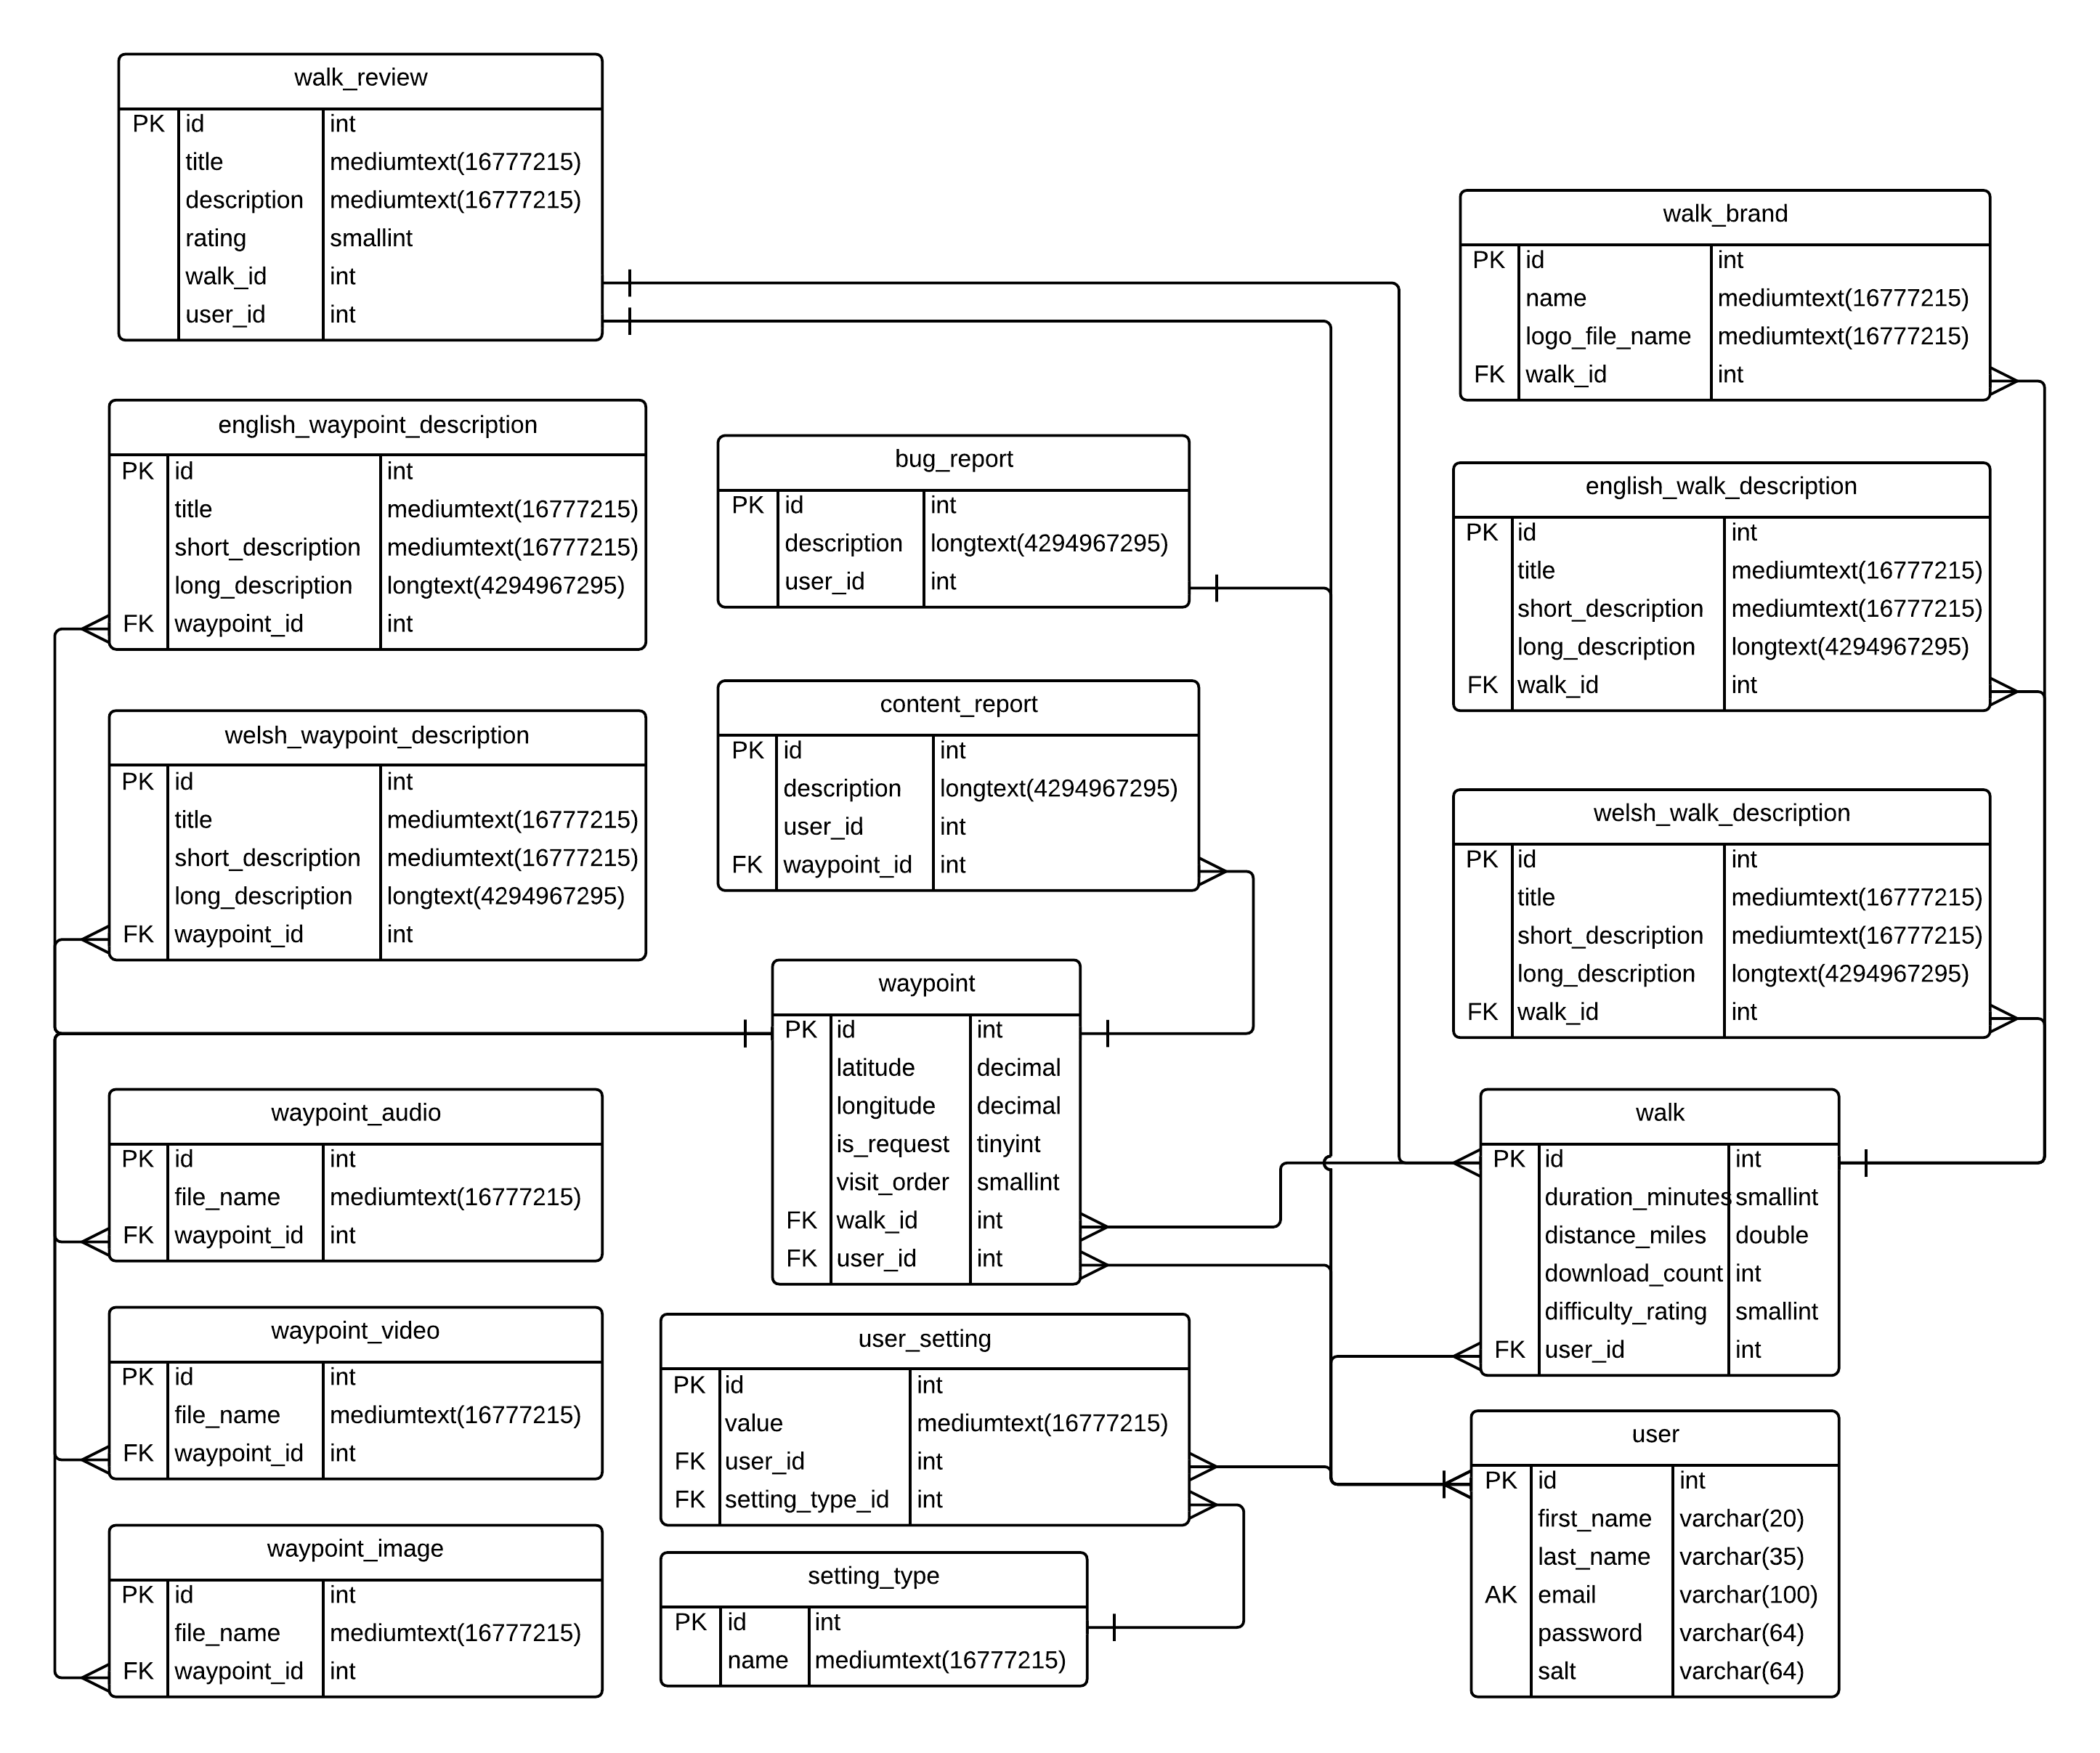
\includegraphics[width=\textwidth]{DatabaseSchema}
    \caption{The Database Schema}
    \label{fig:databaseschema}
\end{figure}

The database is shown in Figure \ref{fig:databaseschema}. It was designed in 3rd Normal Form to reduce data duplication and ensure that integrity through keys. Tables are related by their primary key, called id. If a table is dependent on another table it can use a forign key column which referances the primary key of the secondary table. This design was chosen becouse it allows for the expansion of the database and it ensures the integrity and stability of the data. There was the possibility of progressing the database to a higher normal form, however the work to achive this would out weight any perfomance benifits and the database in 3rdNF nicely matches the structure of the API.

\subsection{Tables}

\subsubsection{walk}
The walk table holds all of the data directly related to a walk. It has a primary key \textit{id}, and a foreign key \textit{user\_id} which relates the walk to the user who owns it by the user's \textit{id} feild. 

\subsubsection{waypoint}
The waypoint table stores all waypoints. Each waypoint has a unique \textit{id} as its primary key, a foreign key \textit{user\_id} which links it to the creater via there own \textit{id} and a foreign key \textit{walk\_id} which relates the waypoint to a specifc walk by the walks unique \textit{id} field. 

\subsubsection{user}
The user table holds all registered users. Every user is assigned a unique \textit{id} as its primary key for relations. The `email' field is designated a `Unique Index' meaning that no two users can have the same email address. 

\subsubsection{walk\_review}
The walk reviews table hold users reviews of a walk. As normal each review gets a unique \textit{id} as its primary key. Reviews then have foriegn keys for \textit{user\_id} and \textit{walk\_id} which relate it to the correct walk and user. 

\subsubsection{walk\_brand}
The walk brand holds some style information for a walk. It has a primary key \textit{id} and is linked to the walk by the foriegn key \textit{walk\_id}. 

\subsubsection{english\_walk\_description}
The english walk description table holds the english version of the walk description. Its mapped to a particular walk through the foriegn key \textit{walk\_id}. It has its own priamry key \textit{id} which is unique to that english walk description. 

\subsubsection{welsh\_walk\_description}
The welsh walk description table holds the welsh version of the walk description. Its mapped to a particular walk through the foriegn key \textit{walk\_id}. It has its own priamry key \textit{id} which is unique to that welsh walk description. 

\subsubsection{english\_waypoint\_description}
The english waypoint description table holds the english version of the waypoint description. Its mapped to a particular walk through the foriegn key \textit{waypoint\_id}. It has its own priamry key \textit{id} which is unique to that english waypoint description. 

\subsubsection{welsh\_waypoint\_description}
The welsh waypoint description table holds the welsh version of the waypoint description. Its mapped to a particular walk through the foriegn key \textit{waypoint\_id}. It has its own priamry key \textit{id} which is unique to that welsh waypoint description. 

\subsubsection{waypoint\_audio}
The waypoint audio table holds information about audio files. They are mapped to the waypoints which they belong to via the foriegn key \textit{waypoint\_id} and have their own primary key \textit{id}.

\subsubsection{waypoint\_image}
The waypoint image table holds information about image files. They are mapped to the waypoints which they belong to via the foriegn key \textit{waypoint\_id} and have their own primary key \textit{id}.

\subsubsection{waypoint\_video}
The waypoint video table holds information about video files. They are mapped to the waypoints which they belong to via the foriegn key \textit{waypoint\_id} and have their own primary key \textit{id}.

\subsubsection{user\_setting}
The users settings table hold the value of each setting for each user. Each row is a specific settings values mapped to a setting type by \textit{setting\_type\_id} and to the user by \textit{user\_id}. Each row has a unique id given by the primary key field \textit{id}.

\subsubsection{setting\_type}
The setting type table stores all the settings a user can have. Each one has a unique \textit{id} as its primary key which is used by user\_settings to assign settings to users.

\subsubsection{content\_report}
The Content Report table stores any reports users have filed about a waypoint. The reports have a unique priary key field \textit{id} and are related to the reported waypoint via a foriegn key \textit{waypoint\_id}. 

\subsubsection{bug\_report}
The Bug report table is used to store bugs in the program that are reported by users. They have a unique priary key field \textit{id} and are related to the user who reported it via a foriegn key \textit{user\_id}

\chapter{Testing}
\label{sec:testing}
\section{Unit Testing}
\label{sec:unit-testint}
\section{Acceptance Testing}
\label{sec:acceptance-testint}


\subsection{API}

While there were never any inital specifications for an API acceptance testing for the API was still carried out using the design documents as a guide. This ensured the API not only has all required features, but also acted as an aditonal round of unit testing to prove that all the functions of the API were working correctly. The API was tested using a program called CoocaRestClient which is an OSX program designed specifically for testing REST API's. The program allows the user to enter a URL, select the HTTP method, set the request payload and set any headers that are required. With this it is possible to access every property of the API and test situations which may not occure through normal useage. \\

\label{test:API-T01}
\noindent\textbf{Test Code:} API-T01\\
\textbf{Asserts Specification:} N/A \\ 
\textbf{Criteria:} \begin{itemize}
                     \item The API must allow for the creation of a new user.
                   \end{itemize}  
\textbf{Result:} \textcolor{green}{PASS}\\ 
\textbf{Description:} A \textbf{POST} request was sent to \url{/users} with a valid JSON object representing a user. The user was created in the database and the API returned a JSON user object including a uninque \textit{ID}. If an invalid user object is passed the API returns a \textit{400} status code and the JSON object \lstinline${"error":"Invalid User Object"}$.\\ 

\label{test:API-T02}
\noindent\textbf{Test Code:} API-T02\\
\textbf{Asserts Specification:} N/A \\ 
\textbf{Criteria:} \begin{itemize}
                     \item It must be possible to authenticate with the API to prove the user is a valid user. 
                   \end{itemize}  
\textbf{Result:} \textcolor{green}{PASS}\\ 
\textbf{Description:} Sending a \textbf{POST} request to \url{/sessions} with a JSON object holding a valid username and password will make the API return a full user object with an Authentication Token. If incorrect details are passed a 403 Forbidden error occurs. The auth token can then be used with every request to generate a secure hash. Sending the hash along with a timestamp and the users email in a series of headers will authenticate the user for that particular request. If the hash dosent match what is required the API will return a 403 Forbiden error. \\ 

\label{test:API-T03}
\noindent\textbf{Test Code:} API-T03\\
\textbf{Asserts Specification:} N/A \\ 
\textbf{Criteria:} \begin{itemize}
                     \item It should be possible to request all walks.
                     \item It should be possible to request a walk by its id.
                     \item It should be possible to limit and offset the number of walks requested when selecting all.
                     \item A user shouldnt have to be authenticated to request a walk.
                   \end{itemize}  
\textbf{Result:} \textcolor{green}{PASS}\\ 
\textbf{Description:} Sending a \textbf{GET} request to \url{/walks} returns an array of all of the walk objects. Adding a \textit{`limit'} paramater to the URL restricts the number of results returned and ensure it cannot be over the limit. Adding a \textit{`offset'} parameter in conjunction with a \textit{`limit'}, such as \url{/walks?limit=10&offset=5}, will ensure that the results are both limited and offset. To retrieve a single walk by its ID a request was sent to the route \url{/walks/}\bfurl{id}. This returned a single walk object with the id equal to \bfurl{id}. \\ 

\label{test:API-T04}
\noindent\textbf{Test Code:} API-T04\\
\textbf{Asserts Specification:} N/A \\ 
\textbf{Criteria:} \begin{itemize}
                     \item It should be possible to add a walks with serveral waypoints in one request.
                     \item It should be possible to update a walk and its waypoints in one request.
                     \item It should be possible to remove a walk and all attached data in one request.
                     \item A user is required to be authenticated for all of these requests.
                     \item A user should only be able to update and delete walks they own. 
                   \end{itemize}  
\textbf{Result:} \textcolor{green}{PASS}\\ 
\textbf{Description:} A \textbf{POST} request was sent to \url{/walks} with a JSON walk object containing several waypoints. The API responded with a fully initalised walk object will all unique id's set. It was then possible to request the walk using the returned id. To update the walk a modified version of the inital walk object was sent via a \textbf{PUT} request to \url{/walks/}\bfurl{id}. The API responded with an updated vesion of the walk object from the database. Again the walk can be requested to show the changes. To delete the walk a \textbf{DELETE} request was sent to \url{/walks/}\bfurl{id}. The API resonded with \lstinline${"deleted":true}$. Every request was initally tried with no authentication headers, which in every case casued a 403 Forbidden error from the API. Updating and deleting was then attempted with valid authentication headers, but for a user other than the one who created the walk. This also returned a 403 Forbidden error. Only with correct authentication headers, for the correct user, were the requests accepted and processed by the API.\\

\label{test:API-T05}
\noindent\textbf{Test Code:} API-T05\\
\textbf{Asserts Specification:} N/A \\ 
\textbf{Criteria:} \begin{itemize}
                     \item It should be possible to add a waypoint to a walk you created if you are authenticated. 
                     \item Anyone should be able to request an array of waypoints for a walk, or a specifica waypoint by its id.
                     \item An authenticated user should be able to update a waypoint they created.
                     \item An authenticated user should be able to delete a waypoint they created.                   
                   \end{itemize}  
\textbf{Result:} \textcolor{green}{PASS}\\ 
\textbf{Description:} To add a walk a \textbf{PSOT} request was sent to \url{/walks/}\bfurl{id}\url{/waypoints} with a JSON waypoint object. The API responded with a completed waypoint object with its unique id. This request was attempted with no authentication headers and then when authenticated as the owner of the walk. When no authentications were present the request caused a 403 Forbidden error. The waypoint could then be requested back from the API using the returned id and a \textbf{GET} request to the route \url{/walks/}\bfurl{id}\url{/waypoints/}\bfurl{wid}.  It can also be requested as part of an array of all waypoints for a walk using a \textbf{GET} request to the route \url{/walks/}\bfurl{id}\url{/waypoints}. To update a waypoint a modified waypoint object was sent as a \textbf{PUT} request to \url{/walks/}\bfurl{id}\url{/waypoints/}\bfurl{wid}. If the user had the authentication headers of the owner of the waypoint or walk then they the request was processed correctly and returned the updated waypoint object. If they authentication headers were missing or the user dosent own the walk or waypoint then a 403 Forbidden error is triggered. To delete the waypoint a \textbf{DELETE} request was sent to \url{/walks/}\bfurl{id}\url{/waypoints/}\bfurl{wid}. Again this required the authentication headers of the walk or waypoint owner or it would cause a 403 Forbidden error. \\

\label{test:API-T06}
\noindent\textbf{Test Code:} API-T06\\
\textbf{Asserts Specification:} N/A \\ 
\textbf{Criteria:} \begin{itemize}
                     \item It should be possible to add a waypoint to a walk you havent created if you are authenticated. 
                     \item The waypoint should be added as a request.
                     \item The owner of the walk should be able to approve the request.
                     \item The owner of the walk should be able to reject the request.
                     \item A user should be able to see all pending requests on their walks.
                   \end{itemize}  
                   
\textbf{Result:} \textcolor{green}{PASS}\\ 
\textbf{Description:} A waypoint as added to a walk by sending a \textbf{POST} request containg a waypoint object to \url{/walks/}\bfurl{id}\url{/waypoints}. When the user has valid authentication headers but is not the owner of the walk the API responds with a completed waypoint object, however the `is\_request' property is set to true. This means that the waypoint is not shown in normal \textbf{GET} request to the API. Using the owners authorisation token it was possible to see all requests to their walks by sending a \textbf{GET} request to \url{/users/}\bfurl{id}\url{/pending-requests}. To appove a request the owners authorisation token was used to send a \textbf{POST} request to \url{/walks/}\bfurl{id}\url{/wapoints/}\bfurl{wid}\url{/approve} with the JSON object \lstinline${"approve":true}$. The waypoint now appears in all \textbf{GET} requests it would normally appear in. To reject a request the JSON object \lstinline${"approve":false}$ was used. This returned the object \lstinline${"deleted":true}$ and the waypoint was removed.\\

\label{test:API-T07}
\noindent\textbf{Test Code:} API-T07\\
\textbf{Asserts Specification:} N/A \\ 
\textbf{Criteria:} \begin{itemize}
                     \item An authenticated user should be able to delete only their own account.
                     \item An authenticated user should be able to modify only their own account. 
                   \end{itemize}  
\textbf{Result:} \textcolor{green}{PASS}\\ 
\textbf{Description:} To test the updating of users a \textbf{PUT} request was sent to \url{/users/}\bfurl{id} with an updated user object. When the authentication headers match the user to update the request was processed correctly and returned an updated version of the user object. Whent the authentication headers were missing or incorrect a 403 Forbidden error was raised and the request failed. To test deletion a \textbf{DELETE} request was sent to \url{/users/}\bfurl{id} with the correct headers for the user with the id = \bfurl{id}. The server responded with a \lstinline${"deleted":true}$ object. When the request was repeated using headers for a user other than the one being deleted the request retuned a 403 Forbidden error. \\

\label{test:API-T08}
\noindent\textbf{Test Code:} API-T08\\
\textbf{Asserts Specification:} N/A \\ 
\textbf{Criteria:} \begin{itemize}
                     \item It should be possible to return a user based on an id.
                     \item It should be possible to reutrn an array of all users.
                     \item It should be possible to search to a user by their email or name.
                     \item Users must be authenticated to return any users. 
                   \end{itemize}  
\textbf{Result:} \textcolor{green}{PASS}\\ 
\textbf{Description:} To get a user based on their id a \textbf{GET} request was sent to \url{/users/}\bfurl{id}, this returned the user whos id matched \bfurl{id}. To get all users a \textbf{GET} request was sent to \url{/users}, this returned an array of all of the user accounts. To search by user name a \textbf{GET} request was sent to \url{/users/search/}\bfurl{query} where \bfurl{query} is the email or name to search for. This returned an array of all users that match the query string. All of these requests were carried out both with and without valid authentication headers. Only when the headers are present were they accepted by the API. When they were missing they API returned a 403 error. \\

\label{test:API-T09}
\noindent\textbf{Test Code:} API-T09\\
\textbf{Asserts Specification:} N/A \\ 
\textbf{Criteria:} \begin{itemize}
                     \item Users should be able to add reviews to walks. 
                     \item Anyone should be able to get a review by its id.
                     \item Users should be able to delete a review.
                     \item Anyone should be able to get all reviews for a walk.
                   \end{itemize}  
\textbf{Result:} \textcolor{green}{PASS}\\ 
\textbf{Description:} For this test first a \textbf{POST} request with a review object is sent to \url{/walks/}\bfurl{id}\url{/reviews}. The API responded to this request with a completed review object. The id from this reiview object was then used to request it back from the server using a \textbf{GET} request to \url{/walks/}\bfurl{id}\url{/reviews/}\bfurl{rid}. The API returned the correct review. To delete the review a \textbf{DELETE} request was sent to \url{/walks/}\bfurl{id}\url{/reviews/}\bfurl{rid}, the server responded with a \lstinline${"deleted":true}$ object. To ensure it was deleted a \textbf{GET} request was sent to \url{/walks/}\bfurl{id}\url{/reviews}. This got all the rewviews for the walk with the id = \bfurl{id}. The new review was missing from the array which proves it was successfully deleted. Each request was attempted with both valid and invalid authentication headers. Adding and deleting reviews retunred a 403 Forbidden error if they were attempted without authentication headers, however getting reviews worked correctly without. \\

\label{test:API-T10}
\noindent\textbf{Test Code:} API-T10\\
\textbf{Asserts Specification:} N/A \\ 
\textbf{Criteria:} \begin{itemize}
                     \item Users should be able to add Images to a waypoint.
                     \item Users should be able to add Videos to a waypoint.
                     \item Users should be able to add Audio to a waypoint.
                   \end{itemize}  
\textbf{Result:} \textcolor{green}{PASS}\\ 
\textbf{Description:}To test adding media an image, a video and some audio were sent via a \textbf{POST} request to \url{/walks/}\bfurl{id}\url{/wapoints/}\bfurl{wid}\url{/images}, \url{/walks/}\bfurl{id}\url{/wapoints/}\bfurl{wid}\url{/videos} and \url{/walks/}\bfurl{id}\url{/wapoints/}\bfurl{wid}\url{/audio}. When the images route recieved the image it processed the request and returned an image object with a url to the file. How ever the other files caused the API to produce a 415 error. Similar things happened with the video and audio routes, where they accepted media of the correct type (eg Videos for the videos route and audio for the audio route) but rejected other types with a 415 error. Attempting to upload a file to any route without the correct authorisation resulted in a 403 Forbidden error message. 


\label{test:API-T11}
\noindent\textbf{Test Code:} API-T11\\
\textbf{Asserts Specification:} N/A \\ 
\textbf{Criteria:} \begin{itemize}
                     \item Anyone should be able to get all Images for a waypoint.
                     \item Anyone should be able to get all Videos for a waypoint.
                     \item Anyone should be able to get all Audio for a waypoint.
                     \item Anyone should be able to get an Image by its id.
                     \item Anyone should be able to get a Video by its id.
                     \item Anyone should be able to get Audio by its id.
                   \end{itemize}  
\textbf{Result:} \textcolor{green}{PASS}\\ 
\textbf{Description:} This test was run 3 times, once for images, once for videos and once for audio. It is only listed for images for berevity, however the result was the same for all routes. Sending a \textbf{GET} request to \url{/walks/}\bfurl{id}\url{/wapoints/}\bfurl{wid}\url{/images} returned an array of all images object for the waypoint with the id = \bfurl{wid}}.
To get an image by its id a \textbf{GET} request was sent to \url{/walks/}\bfurl{id}\url{/wapoints/}\bfurl{wid}\url{/images/}\bfurl{img_id} where \bfurl{img_id} is the id of the image to return. The API responded to the request and returned the image object with the url to the actual file. This worked without any authentication headers, as was required.

\label{test:API-T12}
\noindent\textbf{Test Code:} API-T12\\
\textbf{Asserts Specification:} N/A \\ 
\textbf{Criteria:} \begin{itemize}
                     \item Users should be able to delete an Image from a waypoint.
                     \item Users should be able to delete a Video from a waypoint.
                     \item Users should be able to delete Audio from a waypoint.
                   \end{itemize}  
\textbf{Result:} \textcolor{green}{PASS}\\ 
\textbf{Description:} Deleting images, videos and audio reuires the same test to be run for 3 diffrent routes. Only the image test is listed here, but the otheres all produced the same result. A \textbf{DELETE} request was sent to \url{/walks/}\bfurl{id}\url{/wapoints/}\bfurl{wid}\url{/images/}\bfurl{img_id} and the API responded with \lstinline${"deleted":true}$ object. This required authetication headers for a user or the request would respond with a 403 Forbidden error. 

\chapter{User Manual}
\label{sec:user-manual}

\section{API}

\subsection{JSON Data Objects}

When communicating with the API objects are represented in JSON. Each object is listed below. Bare in mind that the `\textit{id}' field and other keys like `\textit{walk\_id}' are set by the API automatically and it will ignore any changes you attempt to make to them. Fields which are set by the API are marked with the comment \lstinline$\\Set by API$. These will not be effected if you try an set them yourself. 

\subsubsection{Walks}
\lstset{language=json,
keywordstyle=\color{Maroon},
commentstyle=\color{OliveGreen},
showstringspaces=false, tabsize=4, breaklines=true, showspaces=false, stringstyle=\color{Blue}}

\begin{lstlisting}[captionpos=b, caption=An example JSON Walk Object., label=lst:walk]
{
  "id" : "45", \\Set by API
  "english_description" : {},
  "distance_miles" : "12",
  "cover_url" : "",
  "waypoints" : [],
  "brand" : "",
  "user_id" : "106", \\Set by API
  "welsh_description" : {},
  "duration_minutes" : "2",
  "user" : {}, \\Set by API
  "difficulty_rating" : "4",
  "download_count" : "0" \\Set by API
}
\end{lstlisting}

\subsubsection{Waypoints}

\begin{lstlisting}[captionpos=b, caption=An example JSON Waypoint Object., label=lst:walk]
{
  "id" : "5", \\Set by API
  "english_description" : {},
  "longitude" : "-3.93372000",
  "latitude" : "51.63581500",
  "visit_order" : "1",
  "audio" : [],
  "user_id" : "1", \\Set by API
  "is_request" : "0", \\Set by API
  "walk_id" : "1", \\Set by API
  "images" : [],
  "welsh_description" : {},
  "user" : {}, \\Set by API
  "videos" : []
}
\end{lstlisting}

\subsubsection{Users}

\begin{lstlisting}[captionpos=b, caption=An example JSON Waypoint Object., label=lst:walk]
{
    "id" : "1", \\Set by API
    "last_name" : "Barrell",
    "email" : "a.j.3barrell@gmail.com",
    "first_name" : "Adam"
 }
\end{lstlisting}

\subsubsection{Reviews}

\begin{lstlisting}[captionpos=b, caption=An example JSON Waypoint Object., label=lst:walk]
{
    "rating" : "3",
    "id" : "1", \\Set by API
    "title" : "Amazing!",
    "added" : "2014-04-13 12:45:34", \\Set by API
    "description" : "This walk was great fo...r a change.",
    "user_id" : "1", \\Set by API
    "walk_id" : "1" \\Set by API
}
\end{lstlisting}

\subsubsection{Images}

\begin{lstlisting}[captionpos=b, caption=An example JSON Waypoint Object., label=lst:walk]
{
    "waypoint_id" : "5", \\Set by API
    "id" : "1", \\Set by API
    "caption" : "Some caption.",
    "url" : "site_landscape.jpg",
    "thumbnail_url" : "some_thumbnail.jpg"  \\Set by API
}
\end{lstlisting}

\subsubsection{Audio}

\begin{lstlisting}[captionpos=b, caption=An example JSON Waypoint Object., label=lst:walk]
{
    "waypoint_id" : "5", \\Set by API
    "id" : "1", \\Set by API
    "caption" : "The fat cat jumped over the lazy fox. The fat cat jumped over the lazy fox.",
    "url" : "cat.mp3"
}
\end{lstlisting}

\subsubsection{Videos}

\begin{lstlisting}[captionpos=b, caption=An example JSON Waypoint Object., label=lst:walk]
{
    "waypoint_id" : "5", \\Set by API
    "thumbnail_url" : "some_waypoint_thumb.jpg", \\Set by API
    "id" : "1", \\Set by API
    "caption" : "Some caption.",
    "url" : "whiterock.mp4"
}
\end{lstlisting}

\subsection{Walks}

Routes on walks effect walks and all related content, such as waypoints and reviews but not media, which requires a seperate multipart media request. \bfurl{id} represents the walks unique id.

\subsubsection{Getting by id}
\textbf{\textcolor{Maroon}{Method:}} GET\\
\textbf{\textcolor{Maroon}{URL:}} \url{/walks/}\bfurl{id}\\
\textbf{\textcolor{Maroon}{Request Payload:}} N/A\\
\textbf{\textcolor{Maroon}{Response Payload:}} The walk with the id = \bfurl{id}.\\
\textbf{\textcolor{Maroon}{Authorisation Headers Required?:}} No.

\subsubsection{Getting Many}
\textbf{\textcolor{Maroon}{Method:}} GET\\
\textbf{\textcolor{Maroon}{URL:}} \url{/walks}\\
\textbf{\textcolor{Maroon}{Request Payload:}} N/A\\
\textbf{\textcolor{Maroon}{Response Payload:}} An array of all walks.\\
\textbf{\textcolor{Maroon}{Authorisation Headers Required?:}} No.

\subsubsection{Adding}
\textbf{\textcolor{Maroon}{Method:}} POST\\
\textbf{\textcolor{Maroon}{URL:}} \url{/walks}\\
\textbf{\textcolor{Maroon}{Request Payload:}} The walk object to add to the database.\\
\textbf{\textcolor{Maroon}{Response Payload:}} An initialised walk object with its assigned id.\\
\textbf{\textcolor{Maroon}{Authorisation Headers Required?:}} Yes.

\subsubsection{Updating}
\textbf{\textcolor{Maroon}{Method:}} PUT\\
\textbf{\textcolor{Maroon}{URL:}} \url{/walks/}\bfurl{id}\\
\textbf{\textcolor{Maroon}{Request Payload:}} The updated walk object (With the id=\bfurl{id}).\\
\textbf{\textcolor{Maroon}{Response Payload:}} The updaeted walk object from the server.\\
\textbf{\textcolor{Maroon}{Authorisation Headers Required?:}} Yes.

\subsubsection{Deleting}
\textbf{\textcolor{Maroon}{Method:}} DELETE\\
\textbf{\textcolor{Maroon}{URL:}} \url{/walks/}\bfurl{id}\\
\textbf{\textcolor{Maroon}{Request Payload:}} N/A\\
\textbf{\textcolor{Maroon}{Response Payload:}} A confirmation of the deletion \{``success'':true\}.\\
\textbf{\textcolor{Maroon}{Authorisation Headers Required?:}} Yes.

\subsubsection{Searching}
\textbf{\textcolor{Maroon}{Method:}} GET\\
\textbf{\textcolor{Maroon}{URL:}} \url{/walks/search/}\bfurl{query}\\
\textbf{\textcolor{Maroon}{Request Payload:}} N/A\\
\textbf{\textcolor{Maroon}{Response Payload:}} An array of walks where the a field in a descriptio matches the search query.\\
\textbf{\textcolor{Maroon}{Authorisation Headers Required?:}} No.

\subsubsection{Waypoints}

Routes for waypoints effect the waypoint and its descriptions, but not any attached media. \bfurl{id} represents the walks unique id, and \bfurl{wid} represents the waypoints unique id. If a waypoint is added by a user who is not the owner of the walk then it is a added a request which must be approved by the owner of the walk.

\subsubsection{Getting by id}
\textbf{\textcolor{Maroon}{Method:}} GET\\
\textbf{\textcolor{Maroon}{URL:}} \url{/walks/}\bfurl{id}\url{/waypoints/}\bfurl{wid}\\
\textbf{\textcolor{Maroon}{Request Payload:}} N/A\\
\textbf{\textcolor{Maroon}{Response Payload:}} The waypoint with the id = \bfurl{wid}.\\
\textbf{\textcolor{Maroon}{Authorisation Headers Required?:}} No.

\subsubsection{Getting Many}
\textbf{\textcolor{Maroon}{Method:}} GET\\
\textbf{\textcolor{Maroon}{URL:}} \url{/walks/}\bfurl{id}\url{/waypoints}\\
\textbf{\textcolor{Maroon}{Request Payload:}} N/A\\
\textbf{\textcolor{Maroon}{Response Payload:}} An array of the waypoints for the walk with the id = \bfurl{id}.\\
\textbf{\textcolor{Maroon}{Authorisation Headers Required?:}} No.

\subsubsection{Approving a Request}
\textbf{\textcolor{Maroon}{Method:}} POST\\
\textbf{\textcolor{Maroon}{URL:}} \url{/walks/}\bfurl{id}\url{/waypoints/}\bfurl{wid}\url{/approve}\\
\textbf{\textcolor{Maroon}{Request Payload:}} \lstinline${"approve":true}$ or \lstinline${"approve":false}$\\
\textbf{\textcolor{Maroon}{Response Payload:}} A waypoint object\\
\textbf{\textcolor{Maroon}{Authorisation Headers Required?:}} Yes.

\subsubsection{Adding}
\textbf{\textcolor{Maroon}{Method:}} POST\\
\textbf{\textcolor{Maroon}{URL:}} \url{/walks/}\bfurl{id}\url{/waypoints}\\
\textbf{\textcolor{Maroon}{Request Payload:}} The waypoint object to add to the walk with the id = \bfurl{id}.\\
\textbf{\textcolor{Maroon}{Response Payload:}} An initialised waypoint object with its assigned id.\\
\textbf{\textcolor{Maroon}{Authorisation Headers Required?:}} Yes.

\subsubsection{Updating}
\textbf{\textcolor{Maroon}{Method:}} PUT\\
\textbf{\textcolor{Maroon}{URL:}} \url{/walks/}\bfurl{id}\url{/waypoints/}\bfurl{wid}\\
\textbf{\textcolor{Maroon}{Request Payload:}} The updated waypoint object (With the id=\bfurl{wid}).\\
\textbf{\textcolor{Maroon}{Response Payload:}} The updaeted waypoint object from the server.\\
\textbf{\textcolor{Maroon}{Authorisation Headers Required?:}} Yes.

\subsubsection{Deleting}
\textbf{\textcolor{Maroon}{Method:}} DELETE\\
\textbf{\textcolor{Maroon}{URL:}} \url{/walks/}\bfurl{id}\url{/waypoints/}\bfurl{wid}\\
\textbf{\textcolor{Maroon}{Request Payload:}} N/A\\
\textbf{\textcolor{Maroon}{Response Payload:}} A confirmation of the deletion \{``success'':true\}.\\
\textbf{\textcolor{Maroon}{Authorisation Headers Required?:}} Yes.

\subsubsection{Walk Review}

Walk reviews can be added and deleted, but they cannot be modified once they have been added to the database. \bfurl{id} represents the walks unique id, and \bfurl{rid} represents the reviews unique id.

\subsubsection{Getting by id}
\textbf{\textcolor{Maroon}{Method:}} GET\\
\textbf{\textcolor{Maroon}{URL:}} \url{/walks/}\bfurl{id}\url{/reviews/}\bfurl{rid}\\
\textbf{\textcolor{Maroon}{Request Payload:}} N/A\\
\textbf{\textcolor{Maroon}{Response Payload:}} The review with the id = \bfurl{rid}.\\
\textbf{\textcolor{Maroon}{Authorisation Headers Required?:}} No.

\subsubsection{Getting Many}
\textbf{\textcolor{Maroon}{Method:}} GET\\
\textbf{\textcolor{Maroon}{URL:}} \url{/walks/}\bfurl{id}\url{/reviews}\\
\textbf{\textcolor{Maroon}{Request Payload:}} N/A\\
\textbf{\textcolor{Maroon}{Response Payload:}} An array of the reviews for the walk with the id = \bfurl{id}.\\
\textbf{\textcolor{Maroon}{Authorisation Headers Required?:}} No.

\subsubsection{Adding}
\textbf{\textcolor{Maroon}{Method:}} POST\\
\textbf{\textcolor{Maroon}{URL:}} \url{/walks/}\bfurl{id}\url{/reviews}\\
\textbf{\textcolor{Maroon}{Request Payload:}} The review object to add to the walk with the id = \bfurl{id}.\\
\textbf{\textcolor{Maroon}{Response Payload:}} An initialised review object with its assigned id.\\
\textbf{\textcolor{Maroon}{Authorisation Headers Required?:}} Yes.

\subsubsection{Deleting}
\textbf{\textcolor{Maroon}{Method:}} DELETE\\
\textbf{\textcolor{Maroon}{URL:}} \url{/walks/}\bfurl{id}\url{/reviews/}\bfurl{rid}\\
\textbf{\textcolor{Maroon}{Request Payload:}} N/A\\
\textbf{\textcolor{Maroon}{Response Payload:}} A confirmation of the deletion \{``success'':true\}.\\
\textbf{\textcolor{Maroon}{Authorisation Headers Required?:}} Yes.

\subsubsection{Waypoint Image}
Waypoint images can be added and deleted, but they cannot be modified once they have been added to the database. \bfurl{id} represents the walks unique id, \bfurl{wid} represents the waypoints unique id and \bfurl{img_id} represents the images unique id. 

\subsubsection{Getting by id}
\textbf{\textcolor{Maroon}{Method:}} GET\\
\textbf{\textcolor{Maroon}{URL:}} \url{/walks/}\bfurl{id}\url{/waypoints/}\bfurl{wid}\url{/images/}\bfurl{img_id}\\
\textbf{\textcolor{Maroon}{Request Payload:}} N/A\\
\textbf{\textcolor{Maroon}{Response Payload:}} The image with the id = \bfurl{img_id}.\\
\textbf{\textcolor{Maroon}{Authorisation Headers Required?:}} No.

\subsubsection{Getting Many}
\textbf{\textcolor{Maroon}{Method:}} GET\\
\textbf{\textcolor{Maroon}{URL:}} \url{/walks/}\bfurl{id}\url{/waypoints/}\bfurl{wid}\url{/images}\\
\textbf{\textcolor{Maroon}{Request Payload:}} N/A\\
\textbf{\textcolor{Maroon}{Response Payload:}} An array of the images for the waypoint with the id = \bfurl{wid}.\\
\textbf{\textcolor{Maroon}{Authorisation Headers Required?:}} No.

\subsubsection{Adding}
\textbf{\textcolor{Maroon}{Method:}} POST\\
\textbf{\textcolor{Maroon}{URL:}} \url{/walks/}\bfurl{id}\url{/waypoints/}\bfurl{wid}\url{/images}\\
\textbf{\textcolor{Maroon}{Request Payload:}} The image object and the image file in a mult-part upload which will be added to the walk with the walk\_id = \bfurl{id}.\\
\textbf{\textcolor{Maroon}{Response Payload:}} An initialised image object with its assigned id and url of the image.\\
\textbf{\textcolor{Maroon}{Authorisation Headers Required?:}} Yes.

\subsubsection{Deleting}
\textbf{\textcolor{Maroon}{Method:}} DELETE\\
\textbf{\textcolor{Maroon}{URL:}} \url{/walks/}\bfurl{id}\url{/waypoints/}\bfurl{wid}\url{/images/}\bfurl{img_id}\\
\textbf{\textcolor{Maroon}{Request Payload:}} N/A\\
\textbf{\textcolor{Maroon}{Response Payload:}} A confirmation of the deletion \{``success'':true\}.\\
\textbf{\textcolor{Maroon}{Authorisation Headers Required?:}} Yes.


\subsubsection{Waypoint Audio Controller}
Waypoint audio can be added and deleted, but they cannot be modified once they have been added to the database. \bfurl{id} represents the walks unique id, \bfurl{wid} represents the waypoints unique id and \bfurl{aud_id} represents the audios unique id. 

\subsubsection{Getting by id}
\textbf{\textcolor{Maroon}{Method:}} GET\\
\textbf{\textcolor{Maroon}{URL:}} \url{/walks/}\bfurl{id}\url{/waypoints/}\bfurl{wid}\url{/audio/}\bfurl{aud_id}\\
\textbf{\textcolor{Maroon}{Request Payload:}} N/A\\
\textbf{\textcolor{Maroon}{Response Payload:}} The image with the id = \bfurl{aud_id}.\\
\textbf{\textcolor{Maroon}{Authorisation Headers Required?:}} No.

\subsubsection{Getting Many}
\textbf{\textcolor{Maroon}{Method:}} GET\\
\textbf{\textcolor{Maroon}{URL:}} \url{/walks/}\bfurl{id}\url{/waypoints/}\bfurl{wid}\url{/audio}\\
\textbf{\textcolor{Maroon}{Request Payload:}} N/A\\
\textbf{\textcolor{Maroon}{Response Payload:}} An array of the images for the waypoint with the id = \bfurl{wid}.\\
\textbf{\textcolor{Maroon}{Authorisation Headers Required?:}} No.

\subsubsection{Adding}
\textbf{\textcolor{Maroon}{Method:}} POST\\
\textbf{\textcolor{Maroon}{URL:}} \url{/walks/}\bfurl{id}\url{/waypoints/}\bfurl{wid}\url{/audio}\\
\textbf{\textcolor{Maroon}{Request Payload:}} The image object and the image file in a mult-part upload which will be added to the walk with the walk\_id = \bfurl{id}.\\
\textbf{\textcolor{Maroon}{Response Payload:}} An initialised image object with its assigned id and url of the image.\\
\textbf{\textcolor{Maroon}{Authorisation Headers Required?:}} Yes.

\subsubsection{Deleting}
\textbf{\textcolor{Maroon}{Method:}} DELETE\\
\textbf{\textcolor{Maroon}{URL:}} \url{/walks/}\bfurl{id}\url{/waypoints/}\bfurl{wid}\url{/audio/}\bfurl{aud_id}\\
\textbf{\textcolor{Maroon}{Request Payload:}} N/A\\
\textbf{\textcolor{Maroon}{Response Payload:}} A confirmation of the deletion \{``success'':true\}.\\
\textbf{\textcolor{Maroon}{Authorisation Headers Required?:}} Yes.

\subsubsection{Waypoint Video Controller}
Waypoint video can be added and deleted, but they cannot be modified once they have been added to the database. \bfurl{id} represents the walks unique id, \bfurl{wid} represents the waypoints unique id and \bfurl{vid_id} represents the videos unique id. 
 
\subsubsection{Getting by id}
\textbf{\textcolor{Maroon}{Method:}} GET\\
\textbf{\textcolor{Maroon}{URL:}} \url{/walks/}\bfurl{id}\url{/waypoints/}\bfurl{wid}\url{/videos/}\bfurl{vid_id}\\
\textbf{\textcolor{Maroon}{Request Payload:}} N/A\\
\textbf{\textcolor{Maroon}{Response Payload:}} The image with the id = \bfurl{img_id}.\\
\textbf{\textcolor{Maroon}{Authorisation Headers Required?:}} No.

\subsubsection{Getting Many}
\textbf{\textcolor{Maroon}{Method:}} GET\\
\textbf{\textcolor{Maroon}{URL:}} \url{/walks/}\bfurl{id}\url{/waypoints/}\bfurl{wid}\url{/videos}\\
\textbf{\textcolor{Maroon}{Request Payload:}} N/A\\
\textbf{\textcolor{Maroon}{Response Payload:}} An array of the images for the waypoint with the id = \bfurl{wid}.\\
\textbf{\textcolor{Maroon}{Authorisation Headers Required?:}} No.

\subsubsection{Adding}
\textbf{\textcolor{Maroon}{Method:}} POST\\
\textbf{\textcolor{Maroon}{URL:}} \url{/walks/}\bfurl{id}\url{/waypoints/}\bfurl{wid}\url{/videos}\\
\textbf{\textcolor{Maroon}{Request Payload:}} The image object and the image file in a mult-part upload which will be added to the walk with the walk\_id = \bfurl{id}.\\
\textbf{\textcolor{Maroon}{Response Payload:}} An initialised image object with its assigned id and url of the image.\\
\textbf{\textcolor{Maroon}{Authorisation Headers Required?:}} Yes.

\subsubsection{Deleting}
\textbf{\textcolor{Maroon}{Method:}} DELETE\\
\textbf{\textcolor{Maroon}{URL:}} \url{/walks/}\bfurl{id}\url{/waypoints/}\bfurl{wid}\url{/videos/}\bfurl{vid_id}\\
\textbf{\textcolor{Maroon}{Request Payload:}} N/A\\
\textbf{\textcolor{Maroon}{Response Payload:}} A confirmation of the deletion \{``success'':true\}.\\
\textbf{\textcolor{Maroon}{Authorisation Headers Required?:}} Yes.

\subsubsection{User Controller}
Users can be added, which is registration, and retrieve and searched by anyone. However updating and deleting can only be done by the user on their own account.

\subsubsection{Getting by id}
\textbf{\textcolor{Maroon}{Method:}} GET\\
\textbf{\textcolor{Maroon}{URL:}} \url{/users/}\bfurl{id}\\
\textbf{\textcolor{Maroon}{Request Payload:}} N/A\\
\textbf{\textcolor{Maroon}{Response Payload:}} The user with the id = \bfurl{id}.\\
\textbf{\textcolor{Maroon}{Authorisation Headers Required?:}} Yes.

\subsubsection{Getting Many}
\textbf{\textcolor{Maroon}{Method:}} GET\\
\textbf{\textcolor{Maroon}{URL:}} \url{/users}\\
\textbf{\textcolor{Maroon}{Request Payload:}} N/A\\
\textbf{\textcolor{Maroon}{Response Payload:}} An array of all users.\\
\textbf{\textcolor{Maroon}{Authorisation Headers Required?:}} Yes.

\subsubsection{Getting Pending Requests}
\textbf{\textcolor{Maroon}{Method:}} GET\\
\textbf{\textcolor{Maroon}{URL:}} \url{/users/}\bfurl{id}\url{/pending-request}\\
\textbf{\textcolor{Maroon}{Request Payload:}} N/A\\
\textbf{\textcolor{Maroon}{Response Payload:}} An array of waypoints the user needs to approve.\\
\textbf{\textcolor{Maroon}{Authorisation Headers Required?:}} Yes.

\subsubsection{Getting Accepted Requests}
\textbf{\textcolor{Maroon}{Method:}} GET\\
\textbf{\textcolor{Maroon}{URL:}} \url{/users/}\bfurl{id}\url{/request}\\
\textbf{\textcolor{Maroon}{Request Payload:}} N/A\\
\textbf{\textcolor{Maroon}{Response Payload:}} An array of the waypoints the user has contributed.\\
\textbf{\textcolor{Maroon}{Authorisation Headers Required?:}} Yes.

\subsubsection{Adding}
\textbf{\textcolor{Maroon}{Method:}} POST\\
\textbf{\textcolor{Maroon}{URL:}} \url{/users}\\
\textbf{\textcolor{Maroon}{Request Payload:}} The users object to add to the database. With a password feild, un-encrypted.\\
\textbf{\textcolor{Maroon}{Response Payload:}} An initialised user object with its assigned id and an authorisation token.\\
\textbf{\textcolor{Maroon}{Authorisation Headers Required?:}} No.

\subsubsection{Updating}
\textbf{\textcolor{Maroon}{Method:}} PUT\\
\textbf{\textcolor{Maroon}{URL:}} \url{/users/}\bfurl{id}\\
\textbf{\textcolor{Maroon}{Request Payload:}} The updated user object (With the id=\bfurl{id}). Include a password field if you wish to change the password, and a settings array to change a setting.\\
\textbf{\textcolor{Maroon}{Response Payload:}} The updaeted user object from the server.\\
\textbf{\textcolor{Maroon}{Authorisation Headers Required?:}} Yes.

\subsubsection{Deleting}
\textbf{\textcolor{Maroon}{Method:}} DELETE\\
\textbf{\textcolor{Maroon}{URL:}} \url{/users/}\bfurl{id}\\
\textbf{\textcolor{Maroon}{Request Payload:}} N/A\\
\textbf{\textcolor{Maroon}{Response Payload:}} A confirmation of the deletion \{``success'':true\}.\\
\textbf{\textcolor{Maroon}{Authorisation Headers Required?:}} Yes.

\subsubsection{Searching}
\textbf{\textcolor{Maroon}{Method:}} GET\\
\textbf{\textcolor{Maroon}{URL:}} \url{/users/search/}\bfurl{query}\\
\textbf{\textcolor{Maroon}{Request Payload:}} N/A\\
\textbf{\textcolor{Maroon}{Response Payload:}} An array of user where the a field in a username matches the search query.\\
\textbf{\textcolor{Maroon}{Authorisation Headers Required?:}} Yes.

\subsubsection{Session Controller}

The session controller checks passwords and maps authorisation tokesn to user. Login grants the user a token, logout revokes that token. 

\subsubsection{Login}
\textbf{\textcolor{Maroon}{Method:}} POST\\
\textbf{\textcolor{Maroon}{URL:}} \url{/sessions}\\
\textbf{\textcolor{Maroon}{Request Payload:}} The user object with username and password set.\\
\textbf{\textcolor{Maroon}{Response Payload:}} An autherntication token.\\
\textbf{\textcolor{Maroon}{Authorisation Headers Required?:}} No.

\subsubsection{Logout}
\textbf{\textcolor{Maroon}{Method:}} DELETE\\
\textbf{\textcolor{Maroon}{URL:}} \url{/sessions}\\
\textbf{\textcolor{Maroon}{Request Payload:}} N/A\\
\textbf{\textcolor{Maroon}{Response Payload:}} N/A\\
\textbf{\textcolor{Maroon}{Authorisation Headers Required?:}} YES.


\section{Web Portal}

\section{Android Application}

\chapter{Reflective Account}
\label{sec:reflective-account}
\section{Problem Solving}
\label{sec:problem-solving}
\section{Learning Experience}
\label{sec:learning-experience}
\section{Risk Analysis Review}
\label{sec:risk-analysis-review}
\subsection{Anticipated Risks}
\label{sec:anticipated-risks}
\subsection{Un-Anticipated Risks}
\label{sec:unanticipated-risks}
\section{Schedule Review}
\label{sec:schedule-review}
\section{Methodology Review}
\label{sec:methodology-review}
\section{Goals Achieved}
\label{sec:goals-achieved}
\section{Improvements}
\label{sec:improvements}

\chapter*{Summary}
\label{sec:summary}
\addcontentsline{toc}{chapter}{Summary}

%References as subsection
\newpage
\bibliographystyle{plain}
\bibliography{bibliography}

\appendix

\end{document}
